\documentclass[a4paper]{article}
\usepackage{vntex}
%\usepackage[english,vietnam]{babel}
%\usepackage[utf8]{inputenc}
\usepackage{mathptmx}[ptm]
%\usepackage[utf8]{inputenc}
%\usepackage[francais]{babel}
\usepackage{a4wide,amssymb,epsfig,latexsym,array,hhline,fancyhdr}
\usepackage[normalem]{ulem}
%\usepackage{soul}
\usepackage{svg}

\usepackage[makeroom]{cancel}
\usepackage{amsmath}
\usepackage{amsthm}
\usepackage{multicol,longtable,amscd}
\usepackage{diagbox}%Make diagonal lines in tables
\usepackage{booktabs}
\usepackage{alltt}
\usepackage[framemethod=tikz]{mdframed}% For highlighting paragraph backgrounds
\usepackage{caption,subcaption}

\usepackage{lastpage}
\usepackage[lined,boxed,commentsnumbered]{algorithm2e}
\usepackage{enumerate}
\usepackage{color}
\usepackage{graphicx}							% Standard graphics package
\usepackage{array}
\usepackage{tabularx, caption}
\usepackage{multirow}
\usepackage{multicol}
\usepackage{rotating}
\usepackage{graphics}
\usepackage{geometry}
\usepackage{setspace}
\usepackage{epsfig}
\usepackage{tikz}
\usepackage{indentfirst}
\usepackage{float}

\usetikzlibrary{arrows,snakes,backgrounds,calc}
\usepackage[unicode]{hyperref}
\hypersetup{urlcolor=blue,linkcolor=black,citecolor=black,colorlinks=true} 
\usepackage{listings}

%\usepackage{pstcol} 								% PSTricks with the standard color package

\usepackage[normalem]{ulem}

\newtheorem{theorem}{{\bf Định lý}}
\newtheorem{property}{{\bf Tính chất}}
\newtheorem{proposition}{{\bf Mệnh đề}}
\newtheorem{corollary}[proposition]{{\bf Hệ quả}}
\newtheorem{lemma}[proposition]{{\bf Bổ đề}}
\theoremstyle{definition}
\newtheorem{exer}{Bài toán}
\addtocontents{toc}{\protect\thispagestyle{empty}}
% Remove page number in contents page. 
\addtocontents{lof}{\protect\thispagestyle{empty}}
% Remove page number in list of figure page. 
\addtocontents{lot}{\protect\thispagestyle{empty}}
% Remove page number in list of table page. 
\def\thesislayout{	% A4: 210 × 297
	\geometry{
		a4paper,
		total={160mm,240mm},  % fix over page
		left=30mm,
		top=22mm,
            right=20mm,
            bottom=20mm,
	}
}
\def\thesisheadlayout{	% A4: 210 × 297
	\geometry{
		a4paper,
		total={160mm,240mm},  % fix over page
		left=30mm,
		top=10mm,
	}
}
\thesislayout
\lstset{
language=R,
basicstyle=\footnotesize\sffamily,
commentstyle=\ttfamily\color{black},
numbers=left,
numberstyle=\ttfamily\color{black}\footnotesize,
stepnumber=1,
numbersep=5pt,
backgroundcolor=\color{white},
showspaces=false,
showstringspaces=false,
showtabs=false,
frame=single,
tabsize=2,
captionpos=b,
breaklines=true,
breakatwhitespace=false,
title=\lstname,
escapeinside={},
keywordstyle={},
morekeywords={}
}
%\usepackage{fancyhdr}
\setlength{\headheight}{40pt}
\pagestyle{fancy}
\fancyhead{} % clear all header fields
\renewcommand{\footruleskip}{1mm}

\fancyhead[L]{
 \begin{tabular}{rl}
    \begin{picture}(25,15)(0,0)
    \put(0,-8){
\includegraphics[width=10mm, height=10mm]{Images/hcmut.png}}
    %\put(0,-8){\epsfig{width=10mm,figure=hcmut.eps}}
   \end{picture}&
	%
\includegraphics[width=8mm, height=8mm]{hcmut.png} & %
	\begin{tabular}{l}
		\textbf{  Trường Đại Học Bách Khoa - Đại học Quốc gia TP.HCM }\\
		\textbf{  Khoa Khoa Học \& Kỹ Thuật Máy Tính}
	\end{tabular} 	
 \end{tabular}
}
\fancyhead[R]{
	\begin{tabular}{l}
		\tiny \bf \\
		\tiny \bf 
	\end{tabular}  }
\fancyfoot{} % clear all footer fields
\fancyfoot[L]{\scriptsize  Báo cáo Đồ án chuyên ngành(CO4029) - HK1 2024 - 2025}
\fancyfoot[R]{\scriptsize  Trang {\thepage}/\pageref{LastPage}}

\renewcommand{\headrulewidth}{0.3pt}
\renewcommand{\footrulewidth}{0.3pt}

%%%
\setcounter{secnumdepth}{4}
\setcounter{tocdepth}{3}
\makeatletter
\newcounter {subsubsubsection}[subsubsection]
\renewcommand\thesubsubsubsection{\thesubsubsection .\@alph\c@subsubsubsection}
\newcommand\subsubsubsection{\@startsection{subsubsubsection}{4}{\z@}%
                                     {-3.25ex\@plus -1ex \@minus -.2ex}%
                                     {1.5ex \@plus .2ex}%
                                     {\normalfont\normalsize\bfseries}}
\newcommand*\l@subsubsubsection{\@dottedtocline{3}{10.0em}{4.1em}}
\newcommand*{\subsubsubsectionmark}[1]{}
\makeatother

\everymath{\color{black}}%make in-line maths symbols blue to read/check easily

\sloppy
\captionsetup[figure]{labelfont={small,bf},textfont={small,it},belowskip=-1pt,aboveskip=-9pt}
%space remove between caption, figure, and text
\captionsetup[table]{labelfont={small,bf},textfont={small,it},belowskip=-1pt,aboveskip=7pt}
\setlength{\floatsep}{5pt plus 2pt minus 2pt}
\setlength{\textfloatsep}{5pt plus 2pt minus 2pt}
\setlength{\intextsep}{10pt plus 2pt minus 2pt}

\thesislayout

\begin{document}

\begin{titlepage}
\begin{tikzpicture}[remember picture, overlay]
  \draw[line width = 4pt] ($(current page.north west) + (0.4in,-0.5in)$) rectangle ($(current page.south east) + (-0.4in,0.5in)$);
  \draw[line width=1.5pt]
    ($ (current page.north west) + (0.45in,-0.55in) $)
    rectangle
    ($ (current page.south east) + (-0.45in,0.55in) $);
\end{tikzpicture}

\begin{center}
\LARGE \textbf{ĐẠI HỌC QUỐC GIA THÀNH PHỐ HỒ CHÍ MINH} \\
\vspace{0.2cm}
\LARGE \textbf{TRƯỜNG ĐẠI HỌC BÁCH KHOA} \\
\vspace{0.2cm}
\LARGE \textbf{KHOA KHOA HỌC VÀ KỸ THUẬT MÁY TÍNH}
\end{center}

\vspace{0.3cm}

\begin{figure}[h!]
\begin{center}

\includegraphics[width=4cm]{Images/hcmut.png}
\end{center}
\end{figure}

\begin{center}
\begin{tabular}{c}
\multicolumn{1}{c}{\textbf{{\LARGE BÁO CÁO}}}\\
\\{\textbf{{\LARGE ĐỒ ÁN CHUYÊN NGÀNH}}}
\\
\\
\textbf{\LARGE Hệ thống Chatbot tư vấn khách hàng}
\\\\
\\ {\Large Ngành: Khoa học Máy tính}
\\
\\
\end{tabular}
\end{center}
\vspace{0.5cm}
\begin{table}[h]
\begin{tabular}{rll}
\hspace{6 cm} &  \textbf{\Large HỘI ĐỒNG:} {\Large ................................}
\\
\\
\hspace{6 cm} &   \textbf{\Large GVHD:} {\Large TS Trương Tuấn Anh}
\\
\\
\hspace{6 cm}  &   \textbf{\Large TKHĐ:} {\Large ................................}
\\
\\
% TKHĐ là THƯ KÝ HỘI ĐỒNG
\hspace{6 cm} &     \textbf{$\;$ $\;$$\;$$\;$$\;$$\;$$\;$$\;$$\;$$\;$$\;$$\;$$\;$$\;$$\;$$\;$$\;$$\;$$\;$$\;$$\;$$\;$$\;$$\;$$\;$$\;$$\;$$\;$$\;$$\;$$\;$$\;$$\;$$\;$ \Large ---o0o---} 
\\
\\
\hspace{6 cm} &   \textbf{\Large SVTH1:} {\Large Nguyễn Đức An (2112737)}
\\
\\
\hspace{6 cm}&   \textbf{\Large SVTH2:}  {\Large Lê Đình Huy (2113481)}
\\
\\
\hspace{6 cm} &   \textbf{\Large SVTH3:}  {\Large Phạm Đức Thắng (2112336)}
\\
\\
\end{tabular}
\end{table}
\vspace{0.5cm}
\begin{center}
{\Large TP. HỒ CHÍ MINH, THÁNG/NĂM (BẢO VỆ) }
\end{center}
\end{titlepage}
%\thispagestyle{empty}
\newpage
%%%%%%%%%%%%%%%%%INTRO%%%%%%%%%%%%%%%%%%%
\section*{Lời cảm ơn}
\thispagestyle{empty}

I like to acknowledge ...

\clearpage
\pagenumbering{arabic}

\section*{Lời cam đoan}
\thispagestyle{empty}

Đồ án của nhóm có tham khảo các tài liệu, bài báo, trang web như được trình bày ở mục tài liệu tham khảo và ở mỗi tham khảo tôi đều trích dẫn nguồn gốc. Nhóm xin cam đoan rằng ngoài những trích dẫn từ các tham khảo trên, toàn bộ nội dung trong báo cáo là do nhóm tự soạn thảo từ những kết quả nghiên cứu của nhóm, không sao chép từ bất kì tài liệu nào khác.

Nhóm sẽ hoàn toàn chịu xử lý theo quy định nếu có bất cứ sai phạm nào so với
lời cam đoan.

\clearpage
\pagenumbering{arabic}

\section*{Tóm tắt}
\thispagestyle{empty}

I like to acknowledge ...

\clearpage
\pagenumbering{arabic}

\newpage
\tableofcontents
\newpage
\listoffigures
\newpage
\listoftables
\newpage
\setcounter{page}{1}

%%%%%%%%%%%%%%%%%CONTENTS%%%%%%%%%%%%%%%%%%%
\section{Giới thiệu}
\subsection{Đặt vấn đề}

Trong vòng nhiều thế kỷ qua, chúng ta đã chứng kiến sự tăng vọt của lượng dữ liệu người dùng khổng lồ, tạo nền tảng tài nguyên để vận hành các thuật toán học máy và học sâu nhằm xây dựng các hệ thống hướng dữ liệu. Và nổi bật trong các hệ thống như vậy đó chính là các mô hình ngôn ngữ lớn – Large Language model (LLM), có khả năng tạo sinh dữ liệu đáng kinh ngạc đến mức mà các nhà khoa học đương thời gọi chúng là các SOTA (state of the art – tạm dịch Đỉnh cao của công nghệ). Các tác tử hoạt động dựa trên các mô hình đó cũng dần xuất hiện, trong đó, các tác tử đối thoại (conversational agents) hay gọi một cách quen thuộc hơn là các AI chatbot đã dần khẳng định được vị thế của mình trong cộng đồng ứng dụng trí tuệ nhân tạo tạo sinh.

Theo một thống kê thực tế từ đầu năm 2018 của Hubspot, số lượng hàng hóa bán ra cho người dùng trên toàn thế giới thông qua chatbot chiếm tới hơn 47\% và con số này cho đến nay chắc chắn đã lớn hơn rất nhiều. Một báo cáo khác, thực hiện bởi trang Fortune Business Insights, dự đoán thị trường chatbot sẽ tăng từ 396,2 triệu USD (năm 2019) đến 1953,3 triệu USD (năm 2027), tương ứng với tốc độ tăng trưởng CAGR đạt 22.5\%. Con số này đã phần nào chứng minh chatbot đang ngày càng được ứng dụng rộng rãi trong cuộc sống, đặc biệt là trong lĩnh vực kinh doanh. Rất nhiều doanh nghiệp kinh doanh trong lĩnh vực dịch vụ trên toàn cầu đã ưu tiên triển khai chatbot để xử lý hiệu quả tình huống khi nhu cầu khách hàng tăng cao nhưng đội ngũ nhân viên ít ỏi không đủ sức đảm đương.

\begin{figure}[!ht]
    \centering
    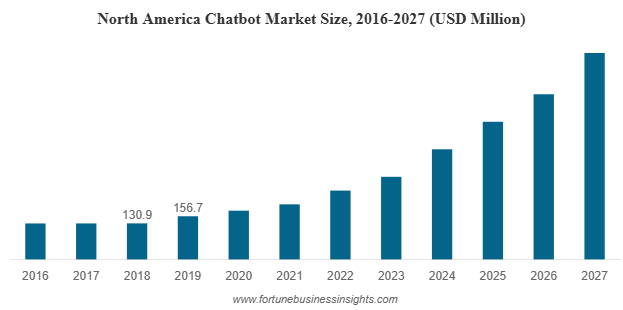
\includegraphics[width=\linewidth]{Images/P1/da2.png}
    \vspace{0.5cm}
    \caption{Thị trường chatbot ở Bắc Mỹ dự đoán đến năm 2027 (triệu USD)}
\end{figure}

Một phân tích khác trên trang web market.us cho biết, phân khúc đám mây đang chiếm giữ thị phần áp đảo so với các hệ thống chatbot on-premise (doanh nghiệp tự triển khai) – chiếm khoảng 64.7\% vào năm 2023. Sự thống lĩnh này phần lớn là nhờ tính linh hoạt, khả năng mở rộng và hiệu quả về chi phí mà các nhà cung cấp giải pháp đám mây đem lại, điều mà các doanh nghiệp rất ưa chuộng, bởi họ có thể dễ dàng mở rộng quy mô các giải pháp chatbot của mình theo nhu cầu khách hàng hiện tại mà không tốn công sức đầu tư cho các hạ tầng máy móc cần thiết. Hơn nữa, chatbot AI dựa trên đám mây được hưởng lợi từ các bản cập nhật và cải tiến liên tục do công nghệ điện toán đám mây tạo ra. Các nhà cung cấp có thể triển khai các bản cập nhật trực tiếp vào cơ sở hạ tầng đám mây, đảm bảo rằng tất cả người dùng đều được hưởng lợi từ những tiến bộ mới nhất trong AI và máy học mà không phải trả thêm chi phí hoặc nỗ lực nào. Vị thế dẫn đầu của phân khúc Đám mây cũng được củng cố bởi sự tin tưởng ngày càng tăng vào các biện pháp bảo mật đám mây và việc áp dụng ngày càng nhiều các môi trường làm việc linh động và từ xa, đòi hỏi các giải pháp linh hoạt và dễ tiếp cận.

\newpage

\begin{figure}[!ht]
    \centering
    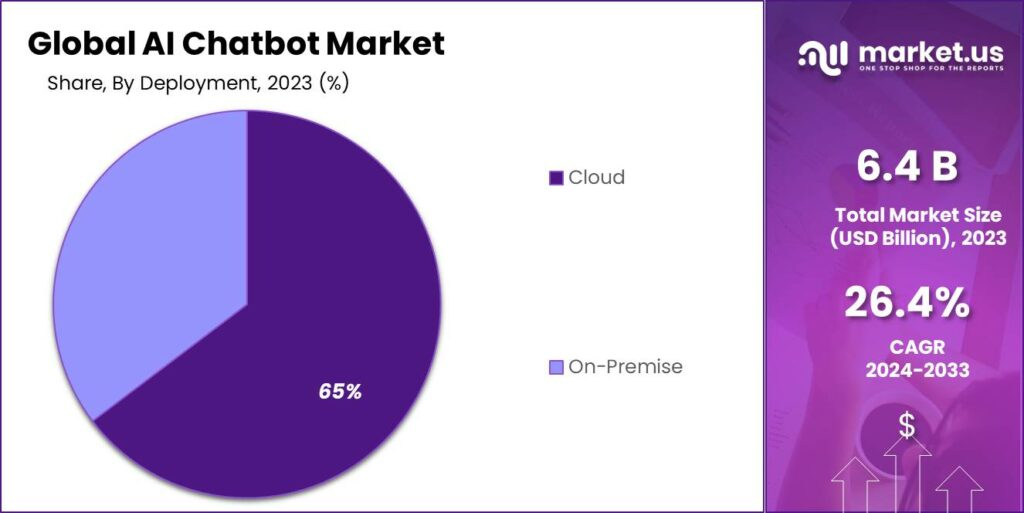
\includegraphics[width=\linewidth]{Images/P1/da3.jpg}
    \vspace{0.5cm}
    \caption{Thị phần chatbot năm 2023 phân theo nơi triển khai}
\end{figure}

Về khía cạnh chọn nền tảng để gắn chatbot vào, Website luôn là ưu tiên hàng đầu bởi chúng chính là mặt tiền kỹ thuật số của một doanh nghiệp và hình ảnh một chatbot với lô gô của doanh nghiệp ở góc dưới cùng bên phải màn hình đã trở thành một điều quen thuộc trong tiềm thức của khách hàng. Ngày nay chatbot hỗ trợ đã trở thành một người bạn đồng hành phổ biến trong hành trình trải nghiệm của người dùng khi truy cập một website thương mại điện tử của doanh nghiệp. Xu hướng này dự kiến sẽ tiếp tục khi ngày càng nhiều các công ty nhận ra tầm quan trọng của việc tăng cường sự tương tác của khách hàng trên các kênh kỹ thuật số chính của họ, khiến các tác tử đối thoại này trở thành một yêu cầu chức năng không thể thiếu khi xây dựng các trang web kinh doanh.

\begin{figure}[!ht]
    \centering
    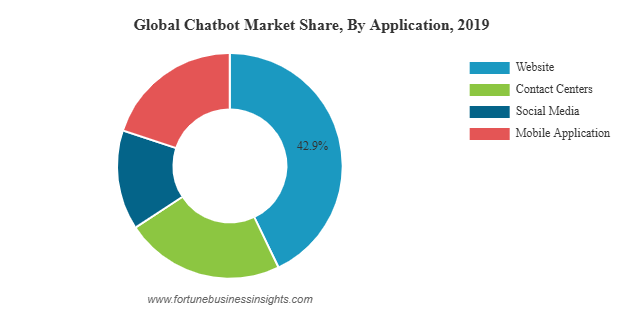
\includegraphics[width=\linewidth]{Images/P1/da1.png}
    \vspace{0.5cm}
    \caption{Thị phần các nền tảng để gắn chatbot năm 2019}
\end{figure}

Các lợi ích của một chatbot hỗ trợ khách hàng:
\begin{itemize}
    \item Tăng tương tác với khách hàng: Với khả năng hoạt động liên tục 24/7, chatbots giúp các doanh nghiệp tương tác hiệu quả với khách hàng mọi lúc mọi nơi. Chúng có thể hỗ trợ đồng thời nhiều khách hàng mà không làm giảm chất lượng dịch vụ và cung cấp phản hồi nhanh chóng đảm bảo khách hàng không phải chờ đợi lâu.
    \item Tự động hóa và tiết kiệm chi phí: Bằng cách tự động hóa các quy trình hỗ trợ, như trả lời các câu hỏi thường gặp, xử lý các yêu cầu đơn giản, doanh nghiệp có thể tiết kiệm nguồn lực đáng kể. Điều này giúp cắt giảm chi phí vận hành, giảm sự phụ thuộc vào lực lượng nhân viên lớn.
    \item Hỗ trợ đa ngôn ngữ: Chatbots có thể được lập trình để hỗ trợ nhiều ngôn ngữ khác nhau, giúp mở rộng phạm vi tương tác với khách hàng từ khắp nơi trên thế giới. Điều này giúp tối ưu hóa trải nghiệm khách hàng toàn cầu và vượt qua rào cản ngôn ngữ, mở rộng thị trường.
    \item Cá nhân hóa trải nghiệm: Với khả năng thu thập và phân tích dữ liệu, chatbot có thể cung cấp các trải nghiệm tương tác được cá nhân hóa cho từng khách hàng, từ đó cải thiện sự hài lòng và lòng trung thành của khách hàng đối với thương hiệu.
    \item Nâng khả năng nhận diện thương hiệu: Chatbots không chỉ là công cụ hỗ trợ, mà còn có thể được thiết kế để phản ánh phong cách và giá trị của thương hiệu. Việc sử dụng chatbot giúp tăng cường nhận diện thương hiệu, làm cho doanh nghiệp trở nên chuyên nghiệp và hiện đại hơn trong mắt khách hàng.
\end{itemize}

Tóm lại, các công nghệ chatbot và mô hình ngôn ngữ lớn	đang trên đà phát triển chóng mặt và việc ứng dụng chúng vào một lĩnh vực cụ thể đó là chăm sóc khách hàng giúp gia tăng lợi ích kinh tế, thăng hạng trang web trong mắt người dùng và tăng cường uy tín của doanh nghiệp trong mắt những khách hàng mới. Nhu cầu phát triển một nền tảng xây dựng chatbot đám mây để phục vụ nhu cầu của doanh nghiệp trở nên bức thiết hơn bao giờ hết, giúp giảm tải khối lượng công việc cho các phòng ban IT của các công ty cũng như chi phí đầu tư cho các hệ thống on-premise.

\subsection{Các hướng giải quyết liên quan}

Với sự gia tăng nhu cầu về dịch vụ hỗ trợ 24/7 và yêu cầu về trải nghiệm cá nhân hóa, các doanh nghiệp cần bổ sung các giải pháp về các chatbot trí tuệ nhân tạo để nâng cao chất lượng dịch vụ khách hàng mà không tốn kém quá nhiều nguồn lực. Chính vì thế, đề tài của nhóm tác giả mong muốn cung cấp dịch vụ tạo chatbot nhằm giúp các doanh nghiệp:

\begin{itemize}
    \item Tiết kiệm thời gian và chi phí: Chatbots tự động hóa các quy trình cơ bản, giúp giảm thiểu chi phí nhân sự và thời gian xử lý yêu cầu.
    \item Cải thiện trải nghiệm khách hàng: Chatbots phản hồi gần như ngay lập tức và cá nhân hóa các tương tác, tạo ấn tượng tốt hơn với khách hàng, qua đó nâng cao tỷ lệ giữ chân khách hàng (Customer Retention Rate – CRR)  
    \item Tăng cường tính cạnh tranh: Trong thị trường cạnh tranh cao, việc áp dụng công nghệ tiên tiến như chatbot giúp doanh nghiệp nổi bật và dễ dàng tiếp cận với khách hàng hơn. Bên cạnh đó, chatbot cũng mang trong mình nhận diện thương hiệu, giúp ghi điểm trong mắt khách hàng qua đó tăng lợi thế cạnh tranh của công ty.
    \item Đón đầu xu hướng: Như đã đề cập, chatbots đang dần trở thành xu hướng toàn cầu, giúp doanh nghiệp không chỉ tối ưu hóa dịch vụ mà còn đi trước đối thủ trong việc áp dụng công nghệ vào quy trình kinh doanh. Công ty hòa nhập trong xu hướng chuyển đổi số của nhà nước, qua đó được tạo điều kiện thuận lơi hơn trên thương trường, mở rộng phạm vi tiếp cận khách hàng.
\end{itemize}

Cụ thể, đề tài hướng đến xây dựng một trang web cung cấp dịch vụ có đăng ký (subscription), cùng giải pháp xây dựng chatbot đám mây hỗ trợ doanh nghiệp nhiều tính năng phổ biến mà không tốn quá nhiều công sức của đội ngũ công nghệ thông tin của công ty hoặc bỏ ra chi phí để xây dựng hạ tầng phần cứng rắc rối. Khi sử dụng ứng dụng này, doanh nghiệp có thể:

\begin{itemize}
    \item Lựa chọn tài liệu phù hợp để huấn luyện chatbot, định dạng text, docs hoặc pdf đều khả dụng
    \item Tùy chỉnh logo, ảnh đại diện, màu sắc, định dạng khung chat nhằm tăng độ nhận diện thương hiệu 
    \item Đội ngũ công nghệ của công ty có thể dễ dàng tích hợp vào app, website của công ty thông qua CDN
    \item Chatbot sẽ được prompting và fine-tuning để tránh việc đưa ra các câu trả lời không phù hợp với tiêu chuẩn đạo đức
    \item Không cần trả thêm bất kỳ khoản chi phí nào khác
\end{itemize}

Đề tài sẽ tập trung vào khả năng tự động hóa các tác vụ hỗ trợ khách hàng, chẳng hạn như trả lời các câu hỏi thường gặp (FAQs), hỗ trợ mua hàng, và xử lý các vấn đề cơ bản và cuối cùng là phân tích sơ lược và thử nghiệm trong một số lĩnh vực thực tế như bán lẻ, dịch vụ để kiểm định tính hiệu quả trong các bối cảnh kinh doanh khác nhau hoặc trong giáo dục, nghiên cứu nhằm kiểm tra tính khả thi về mặt liên ngành. Nhóm tác giả mong muốn kết quả của đề tài này sẽ đóng góp vào việc nghiên cứu và phát triển các ứng dụng liên quan đến AI tạo sinh (Generative AI) cũng như liên quan đến xử lý ngôn ngữ tự nhiên (Natural language processing), từ đó mở rộng hiểu biết của chúng ta về cách thức áp dụng các mô hình ngôn ngữ lớn như một công cụ hiệu quả để tối ưu các tác vụ hỗ trợ người dùng mà cụ thể ở đây là chăm sóc khách hàng.
\newpage
% \section{Cơ sở lý thuyết và công nghệ}
% \subsection{Cơ sở lý thuyết}
% \subsection{Công nghệ}
\section{Nghiên cứu thị trường}
% Tìm hiều về các hệ thống phần mềm tương tự hiện đang có trên thị trường
% Điểm yếu, điểm mạnh -> mục tiêu phát triển phần mềm của mình như thế nào

Hiện nay, trên thị trường quốc tế xuất hiện rất nhiều hệ thống chatbot và các nền tảng hỗ trợ chatbot tư vấn khách hàng. Tuy nhiên, trong phạm vi nghiên cứu này, nhóm tác giả sẽ tập trung phân tích một số hệ thống nổi bật tại thị trường Việt Nam. Mỗi hệ thống đều có những ưu điểm và hạn chế riêng, đi kèm với giao diện thân thiện và bộ tính năng đa dạng, phục vụ cho các nhu cầu khác nhau của doanh nghiệp.
\subsection{AhaChat}
\subsubsection{Giới thiệu}
AhaChat là một nền tảng tạo chatbot phổ biến tại Việt Nam, được thiết kế để hỗ trợ doanh nghiệp tự động hóa quy trình chăm sóc khách hàng và bán hàng qua các kênh như Facebook Messenger, Zalo và Instagram. Với giao diện trực quan và khả năng tạo chatbot không cần lập trình, AhaChat giúp doanh nghiệp dễ dàng thiết lập các kịch bản trò chuyện tự động, từ việc tư vấn sản phẩm, xử lý đơn hàng, đến chăm sóc khách hàng sau bán.

AhaChat được phát triển để giải quyết những thách thức mà nhiều doanh nghiệp gặp phải trong việc duy trì kết nối nhanh chóng và liên tục với khách hàng, đặc biệt qua các nền tảng mạng xã hội như Facebook và Zalo. Nhu cầu tự động hóa các tác vụ như trả lời tin nhắn, xử lý đơn hàng và chăm sóc khách hàng ngày càng trở nên cấp thiết khi số lượng người dùng trực tuyến tăng mạnh. AhaChat ra đời với sứ mệnh hỗ trợ doanh nghiệp giải quyết những vấn đề này thông qua chatbot, giúp tiết kiệm thời gian, chi phí, và tăng cường hiệu quả trong giao tiếp.

\href{https://ahachat.com/}{Link truy cập}
\subsubsection{UI/UX}
\begin{figure}[H]
    \centering
    
\includegraphics[width=1\linewidth]{Images/ahachatlanding.png}
    \vspace{0.5cm}
    \caption{Giao diện trang Landing page của AhaChat}
    \label{fig:enter-label}
\end{figure}
\begin{figure}[H]
    \centering
    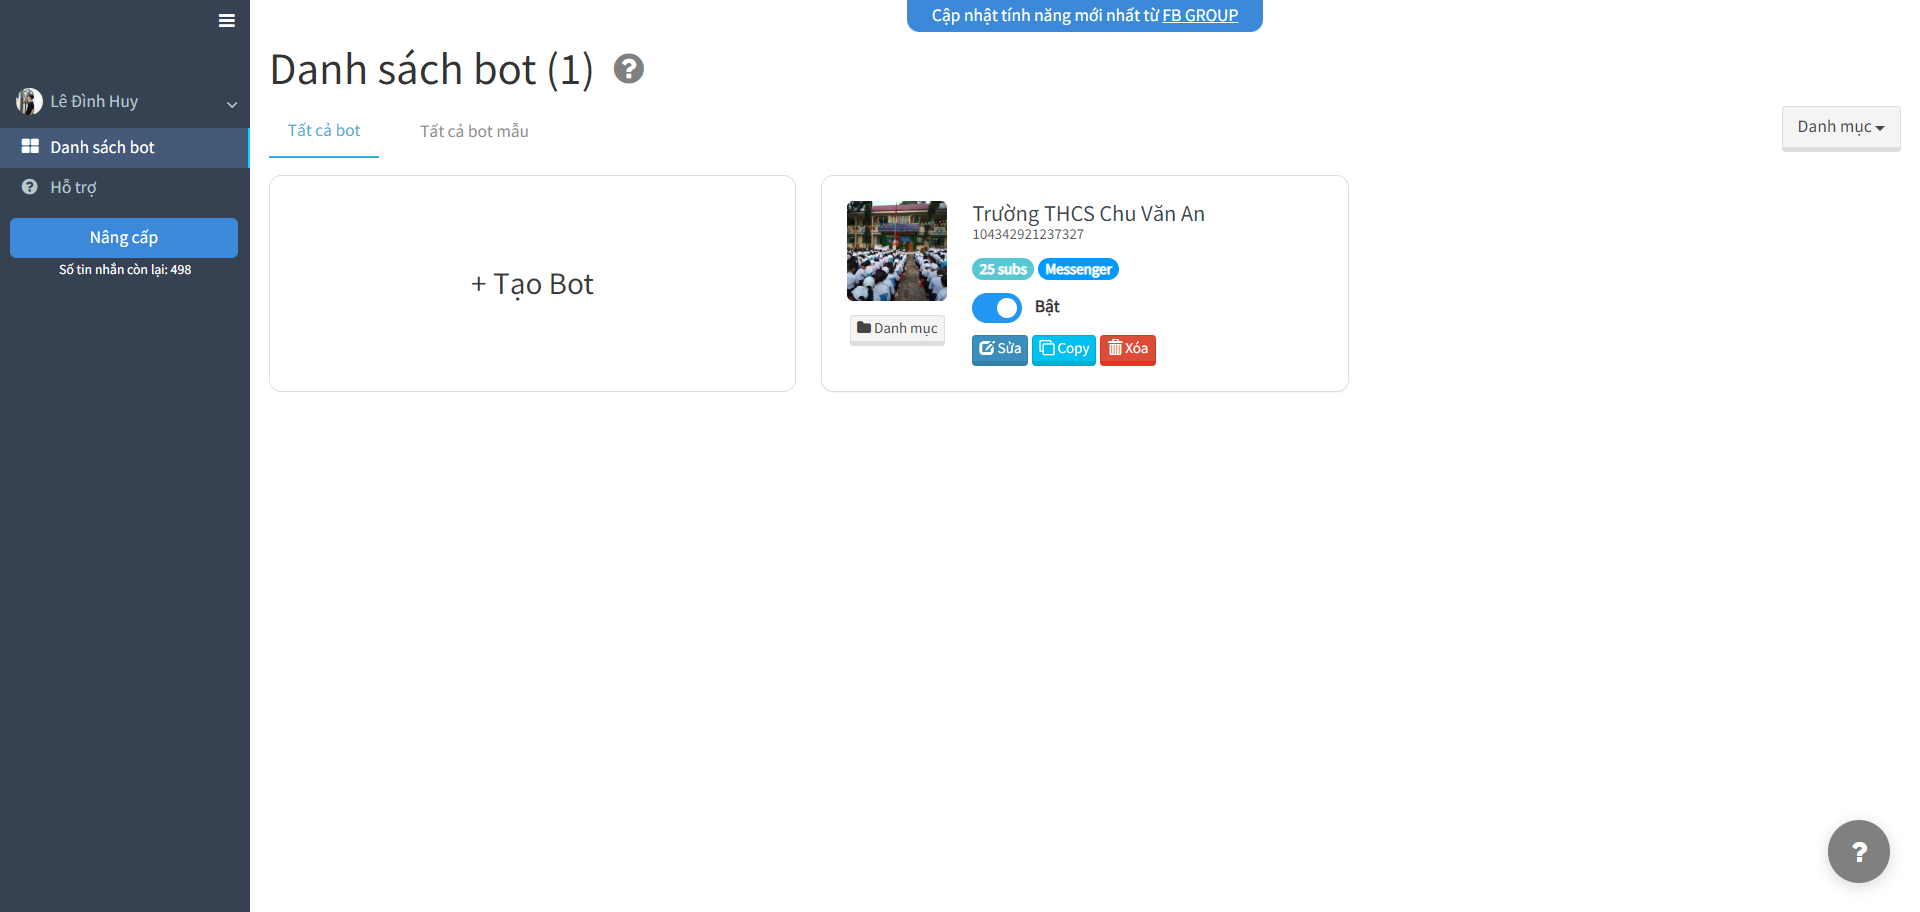
\includegraphics[width=1\linewidth]{Images/homeahachat.png}
    \vspace{0.5cm}
    \caption{Giao diện trang chủ của AhaChat}
    \label{fig:enter-label}
\end{figure}
\begin{figure}[H]
    \centering
    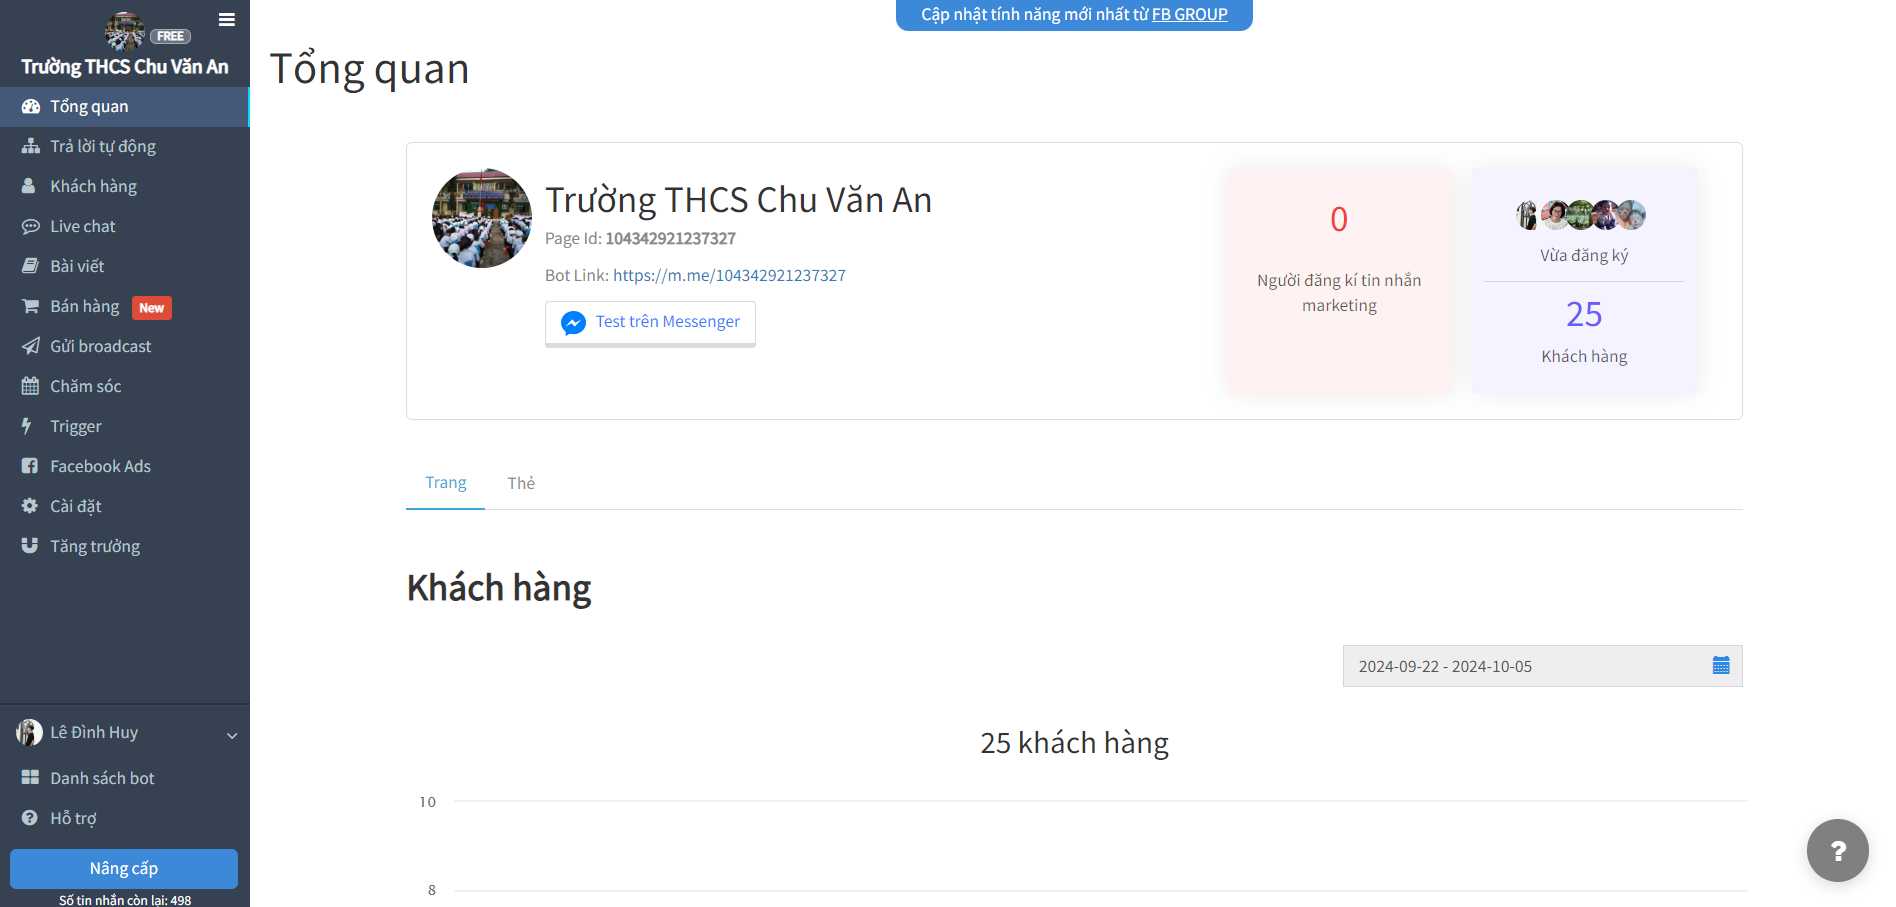
\includegraphics[width=1\linewidth]{Images/quanlypageahachat.png}
    \vspace{0.5cm}
    \caption{Giao diện quản lý fanpage Facebook của AhaChat}
    \label{fig:enter-label}
\end{figure}
\begin{figure}[H]
    \centering
    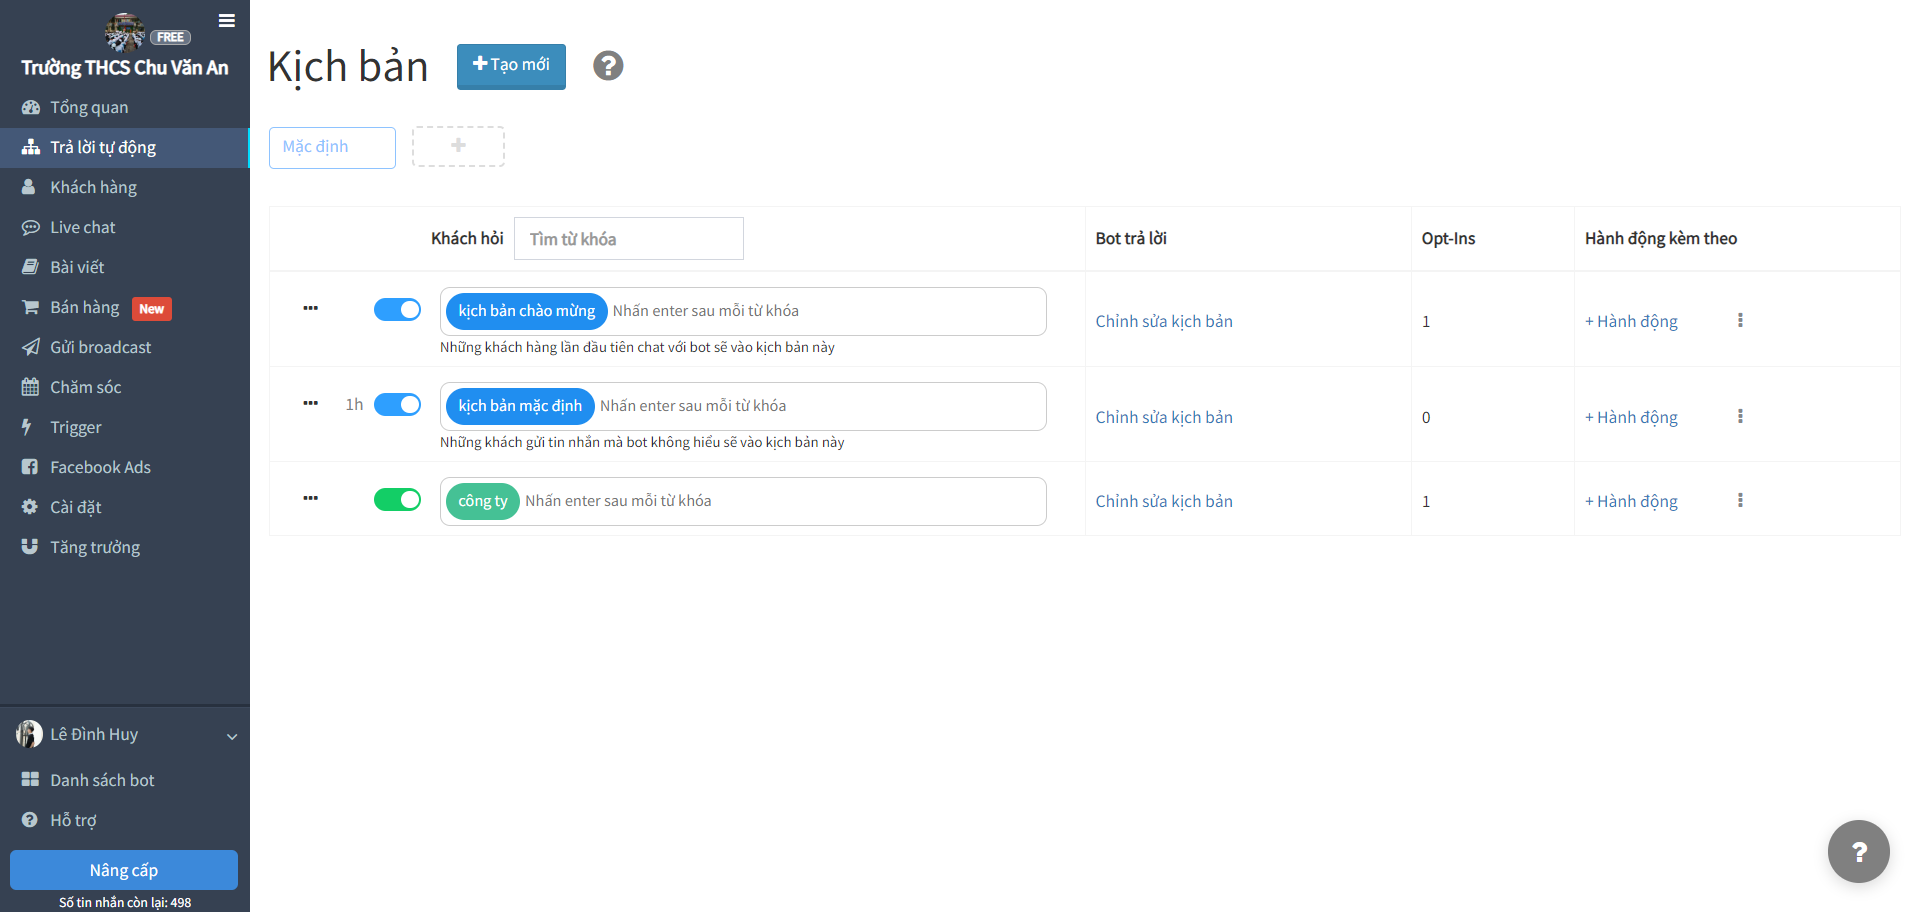
\includegraphics[width=1\linewidth]{Images/quanlykichbanahachat.png}
    \vspace{0.5cm}
    \caption{Giao diện quản lý kịch bản của AhaChat}
    \label{fig:enter-label}
\end{figure}
\subsubsection{Các tính năng chính}
AhaChat là một trong những nền tảng chatbot nổi bật tại Việt Nam, giúp doanh nghiệp tự động hóa giao tiếp và chăm sóc khách hàng hiệu quả. Dưới đây là các tính năng nổi bật giúp tối ưu quy trình bán hàng và tương tác khách hàng trên nhiều kênh trực tuyến.
\begin{itemize}
    \item \textbf{Tạo kịch bản trả lời tự động rất dễ bằng Mind Map:} Người dùng có thể xây dựng kịch bản chatbot một cách trực quan bằng sơ đồ tư duy, giúp dễ dàng tạo ra các cuộc hội thoại logic và hiệu quả.


\item \textbf{Lưu và lấy dữ liệu từ Google Sheets khôi lo sốt đơn:} Tích hợp Google Sheets giúp doanh nghiệp quản lý và theo dõi đơn hàng dễ dàng, không bỏ sót bất kỳ yêu cầu nào từ khách hàng.

\item \textbf{Nhân viên có thể chat trực tiếp với khách thông qua Live Chat:} Tính năng Live Chat cho phép nhân viên chăm sóc khách hàng giao tiếp trực tiếp với khách qua chatbot, tăng cường trải nghiệm khách hàng.

\item \textbf{Phân loại và gửi broadcast hàng loạt để Remarketing:} Doanh nghiệp có thể phân loại khách hàng và gửi tin nhắn hàng loạt cho các chiến dịch tiếp thị lại, giúp thu hút khách hàng tiềm năng quay trở lại.

\item \textbf{Đưa khách hàng vào phễu bằng chiến dịch Chăm sóc:} Quản lý khách hàng theo phễu tiếp thị và chăm sóc tự động, giúp duy trì mối quan hệ lâu dài với khách hàng.

\item \textbf{Auto Inbox để trả lời hàng ngàn comment cùng một lúc:} Chức năng tự động gửi tin nhắn trả lời vào hộp thư của hàng ngàn khách hàng cùng lúc, tiết kiệm thời gian quản lý tương tác.

\item \textbf{Dễ dàng bùng nổ đơn hàng bằng Chatbot Viral:} Sử dụng tính năng chatbot để lan truyền nhanh chóng các thông tin về sản phẩm/dịch vụ, thúc đẩy sự tăng trưởng doanh số.

\item \textbf{Xem thống kê khách hàng và tin nhắn theo thời gian thực:} Công cụ phân tích cho phép theo dõi và báo cáo khách hàng, tình hình tương tác và hiệu suất của chatbot trong thời gian thực.

\item \textbf{Có nhiều công cụ triển khai để tiếp cận khách hàng:} AhaChat cung cấp các công cụ đa dạng giúp doanh nghiệp dễ dàng triển khai các chiến lược tiếp cận và thu hút khách hàng hiệu quả hơn.
\end{itemize}
\begin{figure}[H]
    \centering
    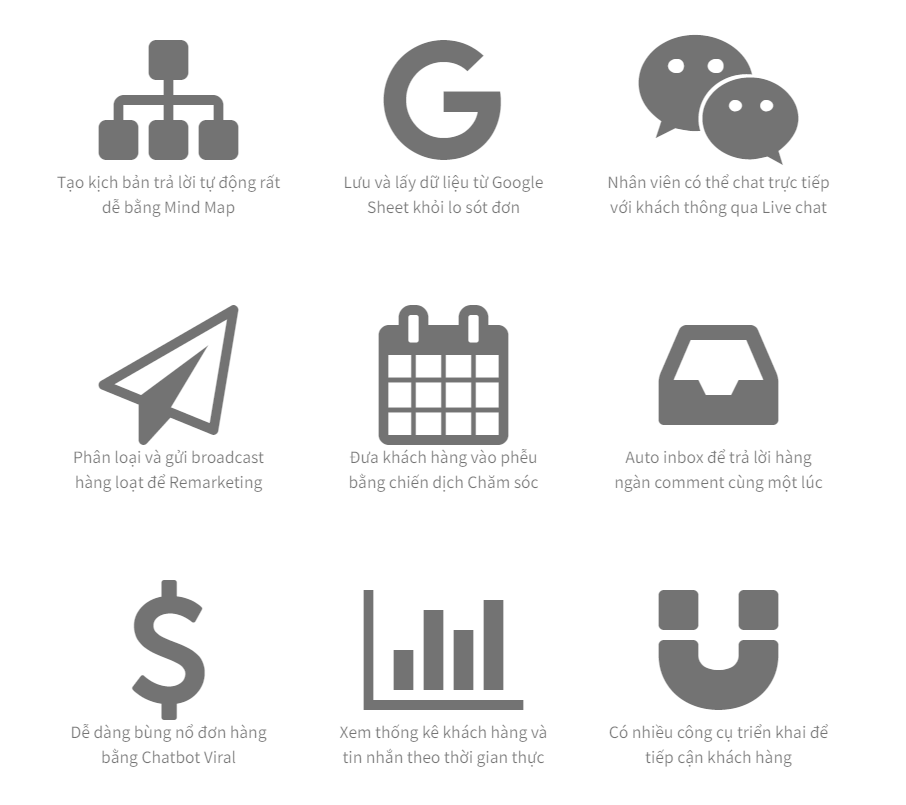
\includegraphics[width=0.75\linewidth]{Images/tinhnangahachat.png}
    \vspace{0.5cm}
    \caption{Giao diện quản lý kịch bản của AhaChat}
    \label{fig:enter-label}
\end{figure}
\subsubsection{Phân tích SWOT}
\begin{table}[H]
\centering
\begin{tabular}{|p{7cm}|p{7cm}|}
\hline
 \begin{center}
     Strengths
 \end{center} & \begin{center}
     Weaknesses
 \end{center}  \\
\hline
\begin{itemize}
    \item Giao diện dễ sử dụng với tính năng kéo-thả Mind Map.
    \item Hỗ trợ tích hợp đa kênh (Facebook,  Messenger, Zalo, Instagram).
    \item Tích hợp công cụ CRM giúp quản lý thông tin khách hàng hiệu quả.
    \item Tính năng tự động hóa quy trình bán hàng và chăm sóc khách hàng mạnh mẽ.
    \item Nhiều công cụ marketing như broadcast, remarketing, và chăm sóc tự động.
\end{itemize} &  
\begin{itemize}
    \item Chỉ tập trung chủ yếu vào thị trường Việt Nam và chưa hỗ trợ chatbot trên website.
\item Khả năng tùy chỉnh nâng cao có thể không đa dạng so với các nền tảng chatbot cao cấp hơn.
\end{itemize}\\
\hline
\begin{center}
    Opportunities
\end{center} & \begin{center}
    Threats
\end{center}\\
\hline
\begin{itemize}
    \item Nhu cầu ngày càng tăng về tự động hóa trong chăm sóc khách hàng và bán hàng trực tuyến tại Việt Nam.
    \item Tiềm năng mở rộng tích hợp với các hệ thống thanh toán, vận chuyển quốc tế.
\end{itemize} &  
\begin{itemize}
    \item Cạnh tranh gay gắt từ các nền tảng mạnh khác ở Việt Nam cũng như quốc tế.
    \item Tốc độ phát triển của công nghệ AI nhanh chóng, yêu cầu cải tiến liên tục để duy trì sự cạnh tranh.
\end{itemize}\\
\hline
\end{tabular}
\caption{Bảng phân tích SWOT cho hệ thống AhaChat}
\end{table}
\subsection{Fchat}
\subsubsection{Giới thiệu}
Fchat phát triển bởi Công ty Cổ phần SaleMall (SaleMall JSC) - đơn vị chuyên về các phần mềm quản lý bán hàng, chăm sóc khách hàng và hệ thống marketing. SaleMall nằm trong hệ sinh thái của Inet Group - tập đoàn hơn 18 năm hoạt động với hệ sinh thái đa dạng về công nghệ thông tin từ tên miền, hosting, VAT, website, đào tạo trực tuyến...

Theo đại diện SaleMall, cùng với sự phát triển mạnh mẽ của thương mại điện tử Việt Nam trong những năm gần đây, doanh nghiệp bán hàng luôn tìm kiếm giải pháp giao tiếp hiệu quả trên các nền tảng mạng xã hội, sàn thương mại điện tử, website... Công nghệ mang lại những cơ hội mới nhưng cũng ra tạo thách thức với chủ kinh doanh nếu không cập nhật kịp thời.

Để giải quyết khó khăn của những nhà bán hàng, Fchat mang đến giải pháp chăm sóc khách hàng hiệu quả hơn. Phần mềm chatbot có khả năng tự động trả lời câu hỏi 24/7, hỗ trợ trả lời tin nhắn và chăm sóc hàng nghìn người cùng một lúc mà không bị gián đoạn. Điều này giúp Fchat trở thành công cụ hỗ trợ hiệu quả cho doanh nghiệp kinh doanh online.

\href{https://fchat.vn/}{Link truy cập}
\subsubsection{UI/UX}
\begin{figure}[H]
    \centering
    
\includegraphics[width=1\linewidth]{Images/landingfchat.png}
    \vspace{0.5cm}
    \caption{Giao diện trang Landing page của Fchat}
    \label{fig:enter-label}
\end{figure}
\begin{figure}[H]
    \centering
    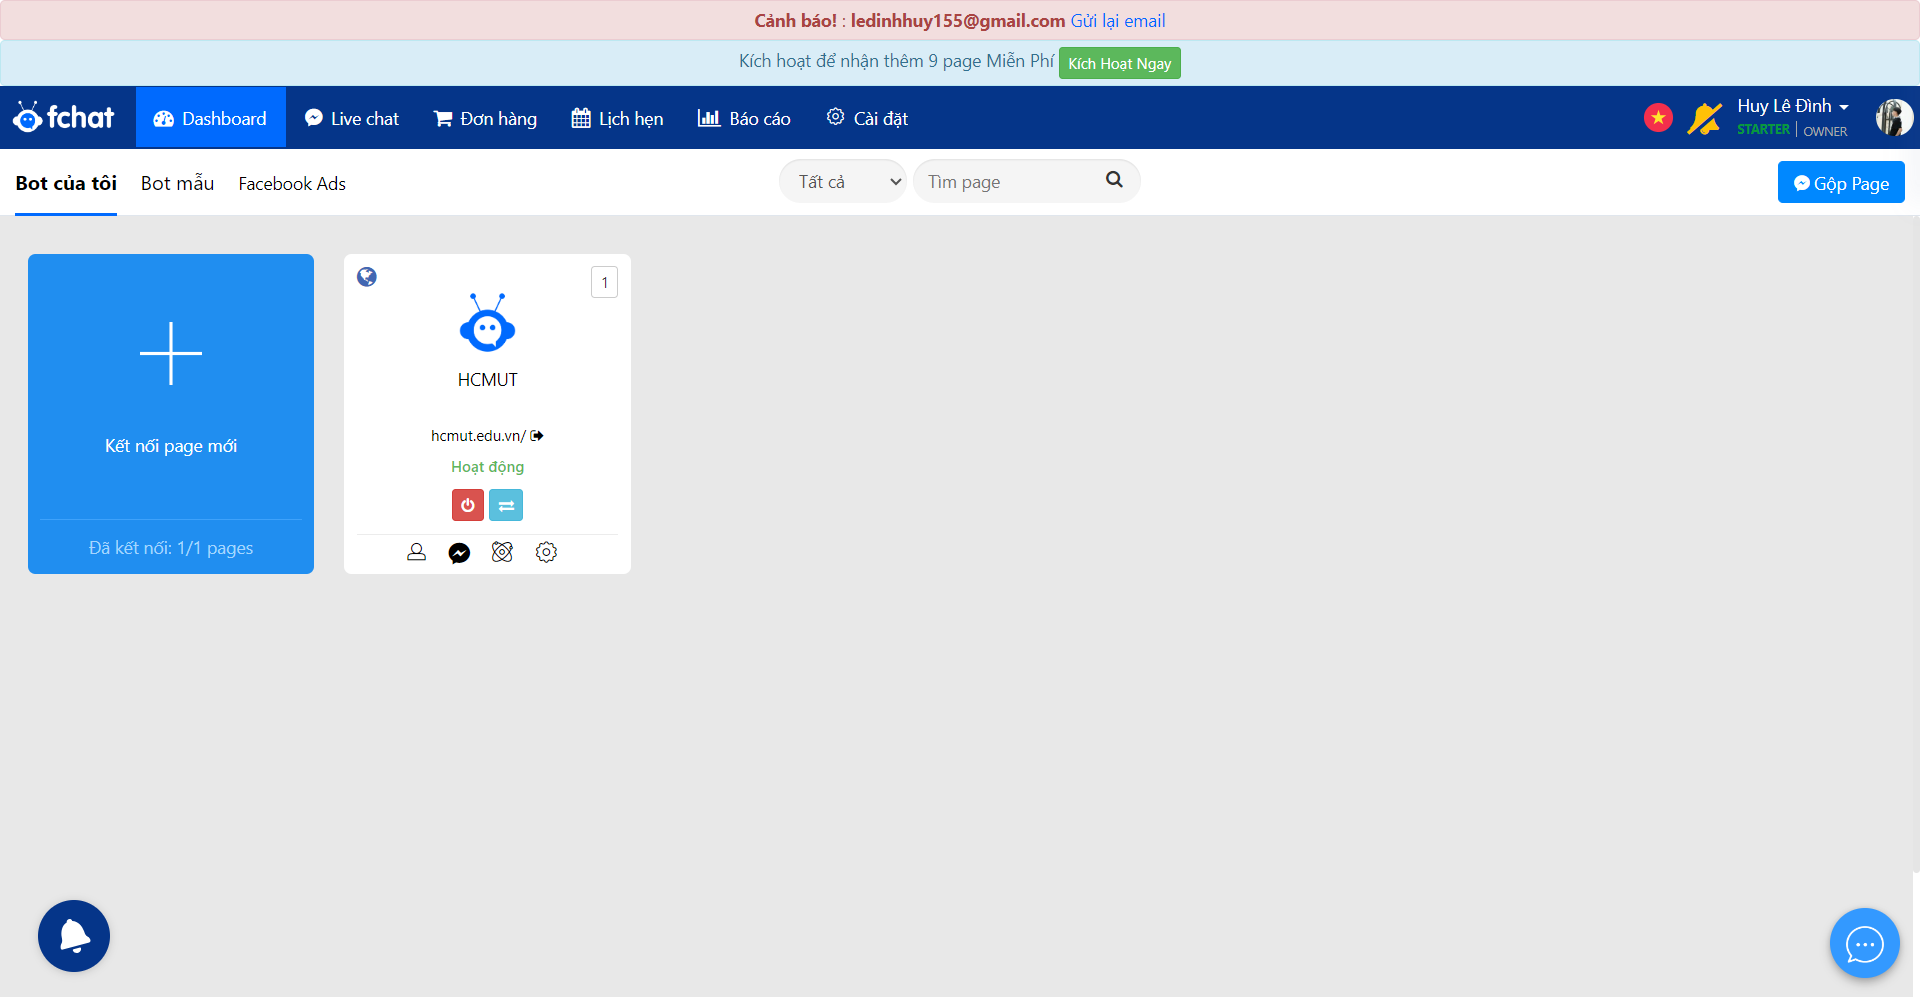
\includegraphics[width=1\linewidth]{Images/fchatdashboard.png}
    \vspace{0.5cm}
    \caption{Giao diện trang Dashboard của Fchat}
    \label{fig:enter-label}
\end{figure}
\begin{figure}[H]
    \centering
    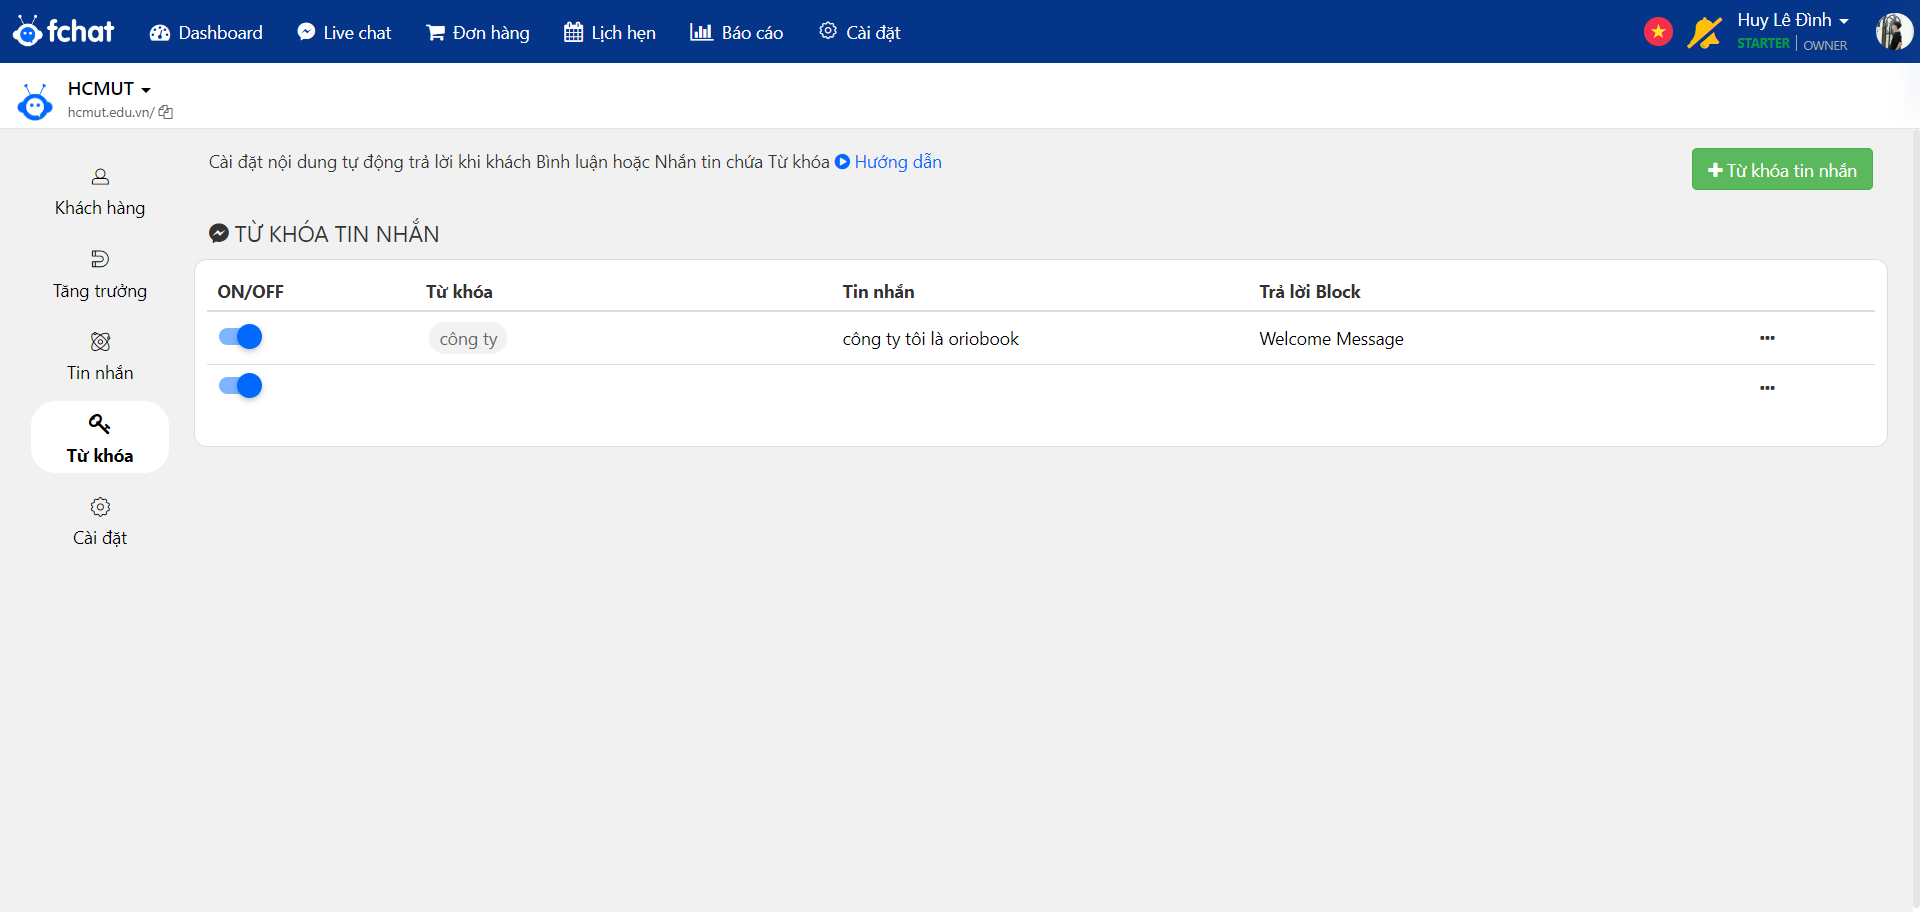
\includegraphics[width=1\linewidth]{Images/tukhoafchat.png}
    \vspace{0.5cm}
    \caption{Giao diện quản lý từ khóa tin nhắn của Fchat}
    \label{fig:enter-label}
\end{figure}
\begin{figure}[H]
    \centering
    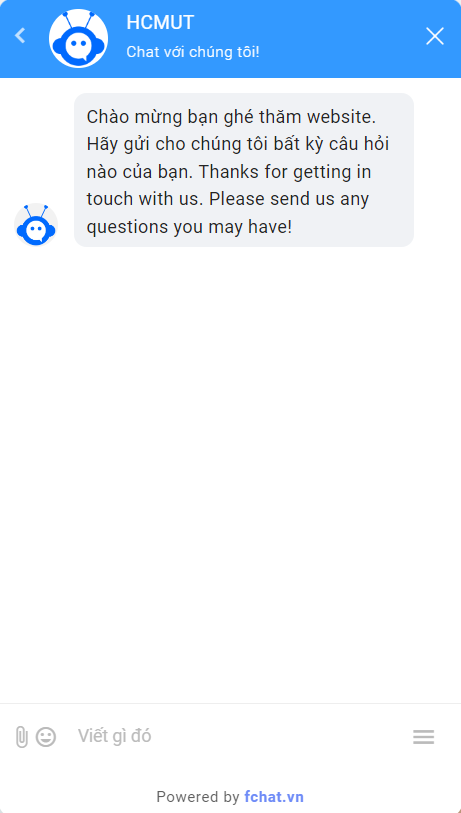
\includegraphics[width=0.5\linewidth]{Images/chatfchat.png}
    \vspace{0.5cm}
    \caption{Giao diện khung chat của Fchat}
    \label{fig:enter-label}
\end{figure}
\subsubsection{Các tính năng chính}
Fchat là một nền tảng chatbot dành cho doanh nghiệp, tập trung vào việc tự động hóa giao tiếp với khách hàng thông qua Facebook Messenger và các kênh khác. Dưới đây là các tính năng chính và mô tả về Fchat:

\begin{itemize}
    \item \textbf{Tự động trả lời tin nhắn:} Fchat cho phép thiết lập chatbot tự động trả lời các tin nhắn từ khách hàng trên Facebook Messenger, giúp doanh nghiệp phản hồi nhanh chóng và không bị gián đoạn.
    
    \item \textbf{Tự động bình luận và trả lời bình luận trên bài viết:} Chatbot Fchat có thể tự động trả lời bình luận của khách hàng trên các bài viết Facebook, đồng thời gửi tin nhắn riêng (inbox) để tiếp tục tư vấn hoặc quảng bá sản phẩm.
    \item \textbf{Gửi tin nhắn hàng loạt (Broadcasting):} Fchat hỗ trợ tính năng gửi tin nhắn hàng loạt đến nhiều khách hàng cùng lúc, giúp doanh nghiệp tiếp thị và quảng bá sản phẩm hiệu quả.

    \item \textbf{Tạo lịch hẹn và tự động nhắc nhở:} Fchat hỗ trợ chức năng tạo lịch hẹn với khách hàng ngay trong hội thoại, đồng thời gửi thông báo nhắc nhở tự động trước số ngày, số giờ tùy chỉnh.

    \item \textbf{Tạo đơn hàng tự động:} Fchat hỗ trợ doanh nghiệp tự động tạo đơn hàng khi khách hàng tương tác qua các kênh như Livestream, quảng cáo, form đặt hàng hoặc trang bán hàng (selling page). Điều này giúp quy trình bán hàng trở nên nhanh chóng và tiện lợi.

    \item \textbf{Kết nối và đồng bộ với các đơn vị vận chuyển:} Fchat có thể kết nối với các đơn vị vận chuyển như Giao Hàng Nhanh, Giao Hàng Tiết Kiệm, Viettel Post, v.v., giúp tự động đồng bộ và quản lý đơn hàng vận chuyển.
    
    \item \textbf{Thống kê và báo cáo chi tiết:} Fchat cung cấp các công cụ thống kê chi tiết về hiệu quả tương tác của chatbot, giúp doanh nghiệp nắm bắt được mức độ hiệu quả của từng chiến dịch và kịch bản.
\end{itemize}
\begin{figure}[H]
    \centering
    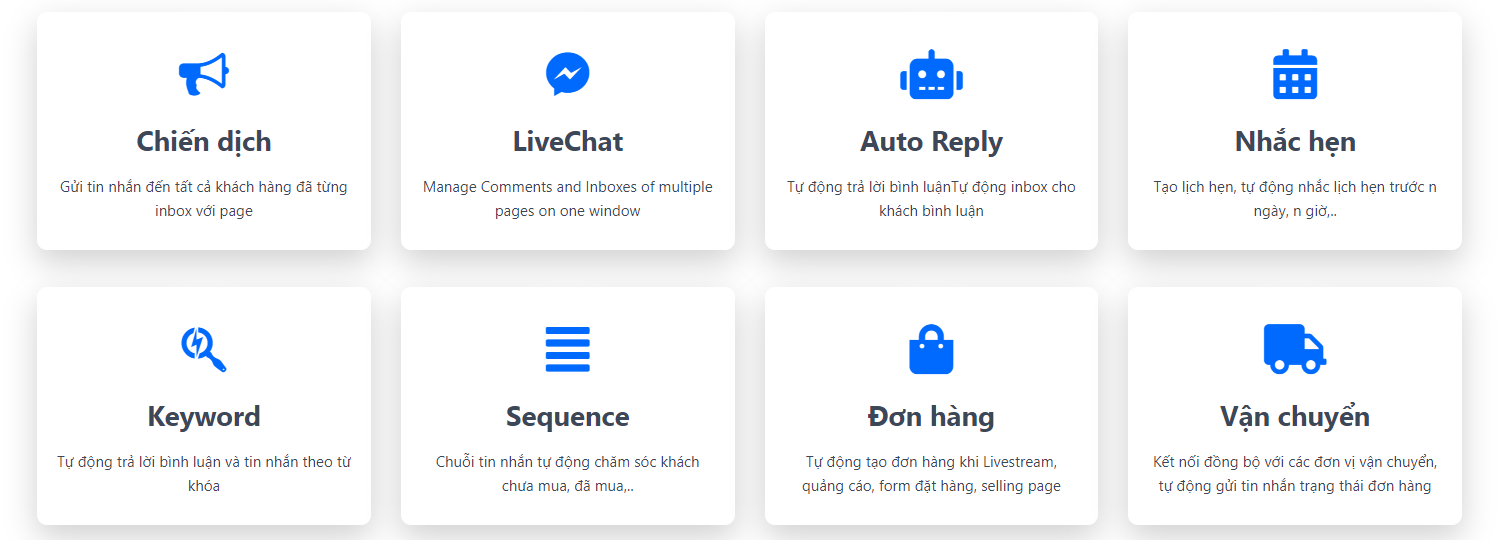
\includegraphics[width=1\linewidth]{Images/featurefchat.png}
    \vspace{0.5cm}
    \caption{Các tính năng cơ bản của Fchat}
    \label{fig:enter-label}
\end{figure}
\subsubsection{Phân tích SWOT}
\begin{table}[H]
\centering
\begin{tabular}{|p{7cm}|p{7cm}|}
\hline
 \begin{center}
     Strengths
 \end{center} & \begin{center}
     Weaknesses
 \end{center}  \\
\hline
\begin{itemize}
    \item Tích hợp tính năng hỗ trợ tự động hóa bán hàng qua Livestream.
    \item Hỗ trợ tạo lịch hẹn và tự động nhắc nhở khách hàng.
    \item Kết nối với các đơn vị vận chuyển và tự động cập nhật trạng thái đơn hàng.
    \item Nền tảng thân thiện với người dùng, dễ dàng tích hợp vào các hệ thống kinh doanh.
\end{itemize} &  
\begin{itemize}
    \item Tập trung vào Facebook Messenger, website, thiếu đa dạng kênh hỗ trợ như Instagram hoặc Zalo.
    \item Quá nhiều tính năng gây phức tạp, khó thể thành thạo trong khoảng thời gian ngắn.
\end{itemize}\\
\hline
\begin{center}
    Opportunities
\end{center} & \begin{center}
    Threats
\end{center}\\
\hline
\begin{itemize}
    \item Tiềm năng lớn trong thị trường livestream bán hàng, đặc biệt tại Việt Nam.
\item Khả năng phát triển các tính năng tích hợp cho doanh nghiệp trong lĩnh vực thương mại điện tử.
\end{itemize} &  
\begin{itemize}
    \item Các nền tảng cạnh tranh khác ngày càng hoàn thiện và cung cấp các tính năng tương tự.
\item Yêu cầu phát triển tính năng mới liên tục để đáp ứng nhu cầu người dùng.
\end{itemize}\\
\hline
\end{tabular}
\caption{Bảng phân tích SWOT cho hệ thống Fchat}
\end{table}
\subsection{TuDongChat}
\subsubsection{Giới thiệu}
TuDongChat là công cụ AI Chatbot sử dụng sức mạnh của trí tuệ nhân tạo nhằm xây dựng những tính năng tự động hàng loạt, thay thế đến 99
\% sức mạnh con người. Với công cụ này, người dùng có thể tích hợp vào bất cứ nền tảng nào như website, Facebook, Zalo một cách dễ dàng mà không cần biết về kiến thức lập trình.


Được phát triển bởi công ty Anthropic, một trong những công ty dẫn đầu về công nghệ trí tuệ nhân tạo. TuDongChat ra mắt vào tháng 6/2022 với sứ mệnh cung cấp giải pháp Chatbot tiện lợi, hiệu quả cho các doanh nghiệp. Mặc dù chỉ mới hoạt động trên thị trường được 2 năm, song phần mềm này nhanh chóng nhận được sự quan tâm của đông đảo khách hàng.

\href{https://tudongchat.com/}{Link truy cập}
\subsubsection{UI/UX}
\begin{figure}[H]
    \centering
    
\includegraphics[width=1\linewidth]{Images/uiTuDongChat.png}
    \vspace{0.5cm}
    \caption{Giao diện trang Landing page của TuDongChat}
    \label{fig:enter-label}
\end{figure}

\begin{figure}[H]
    \centering
    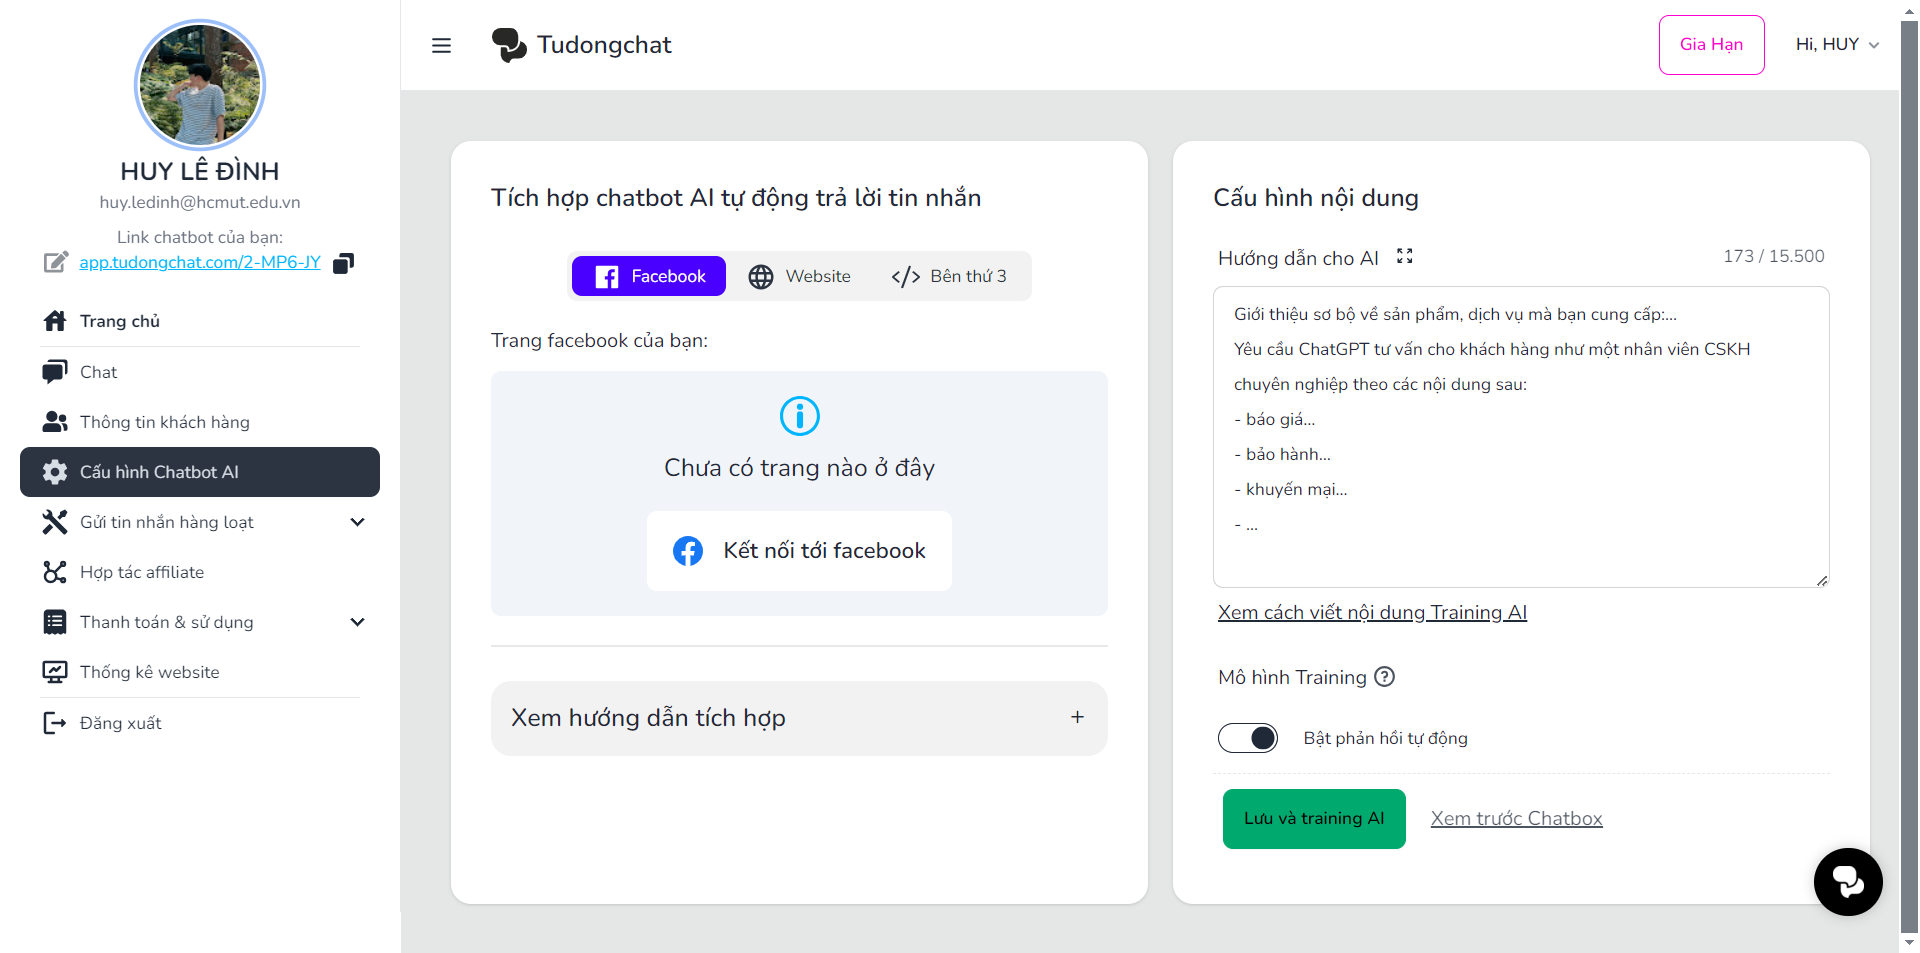
\includegraphics[width=1\linewidth]{Images/uiTuDongChat2.png}
    \vspace{0.5cm}
    \caption{Giao diện Trang chủ của TuDongChat}
    \label{fig:enter-label}
\end{figure}

\begin{figure}[H]
    \centering
    
\includegraphics[width=0.5\linewidth]{Images/uiTuDongChat3.png}
    \vspace{0.5cm}
    \caption{Giao diện khung chat của TuDongChat}
    \label{fig:enter-label}
\end{figure}
\subsubsection{Các tính năng chính}
Với sức mạnh của trí tuệ nhân tạo, TuDongChat cung cấp các tính năng cơ bản sau:
\begin{itemize}
    \item \textbf{Tự động gửi tin hàng loạt:} Giúp doanh nghiệp gửi thông tin tiếp thị cho khách hàng về sản phẩm mới, chương trình khuyến mãi hoặc sự kiện sắp diễn ra. Bằng việc sử dụng trí tuệ nhân tạo để tùy biến thông điệp một cách linh hoạt, không spam, đảm bảo an toàn tuyệt đối cho tài khoản mạng xã hội Facebook \& Zalo của bạn.
    \item \textbf{Tự động tìm kiếm khách hàng tiềm năng:} AI Chatbot TuDongChat không dừng lại ở việc chờ đợi khách hàng liên hệ, mà còn tự động tham gia vào các hội nhóm Facebook, tìm kiếm các bài viết liên quan và tương tác với người dùng tiềm năng, giúp bạn mở rộng mạng lưới khách hàng một cách tự nhiên và linh hoạt.
    \item \textbf{Tự động spam comment Facebook:} AI Chatbot TuDongChat với khả năng đọc hiểu và sáng tạo nội dung theo ngữ cảnh, sẽ giúp bạn spam comment trên các hội nhóm Facebook nhưng vẫn đảm bảo an toàn 100\% cho nick Facebook của bạn.
    \item \textbf{Tự động tương tác và trả lời khách hàng một cách tự nhiên:} Cuối cùng nhưng không kém phần quan trọng, chatbot của chúng tôi không chỉ là một trợ lý cấp cao. Chúng tôi sử dụng trí tuệ nhân tạo ChatGPT để tương tác với khách hàng trên mọi nền tảng – từ website đến fanpage Facebook của bạn. Từ việc trả lời các câu hỏi cơ bản đến việc hỗ trợ mua hàng, chúng tôi đảm bảo rằng mỗi cuộc trò chuyện đều diễn ra một cách tự nhiên và đáp ứng nhanh chóng.
\end{itemize}
\begin{figure}[H]
    \centering
    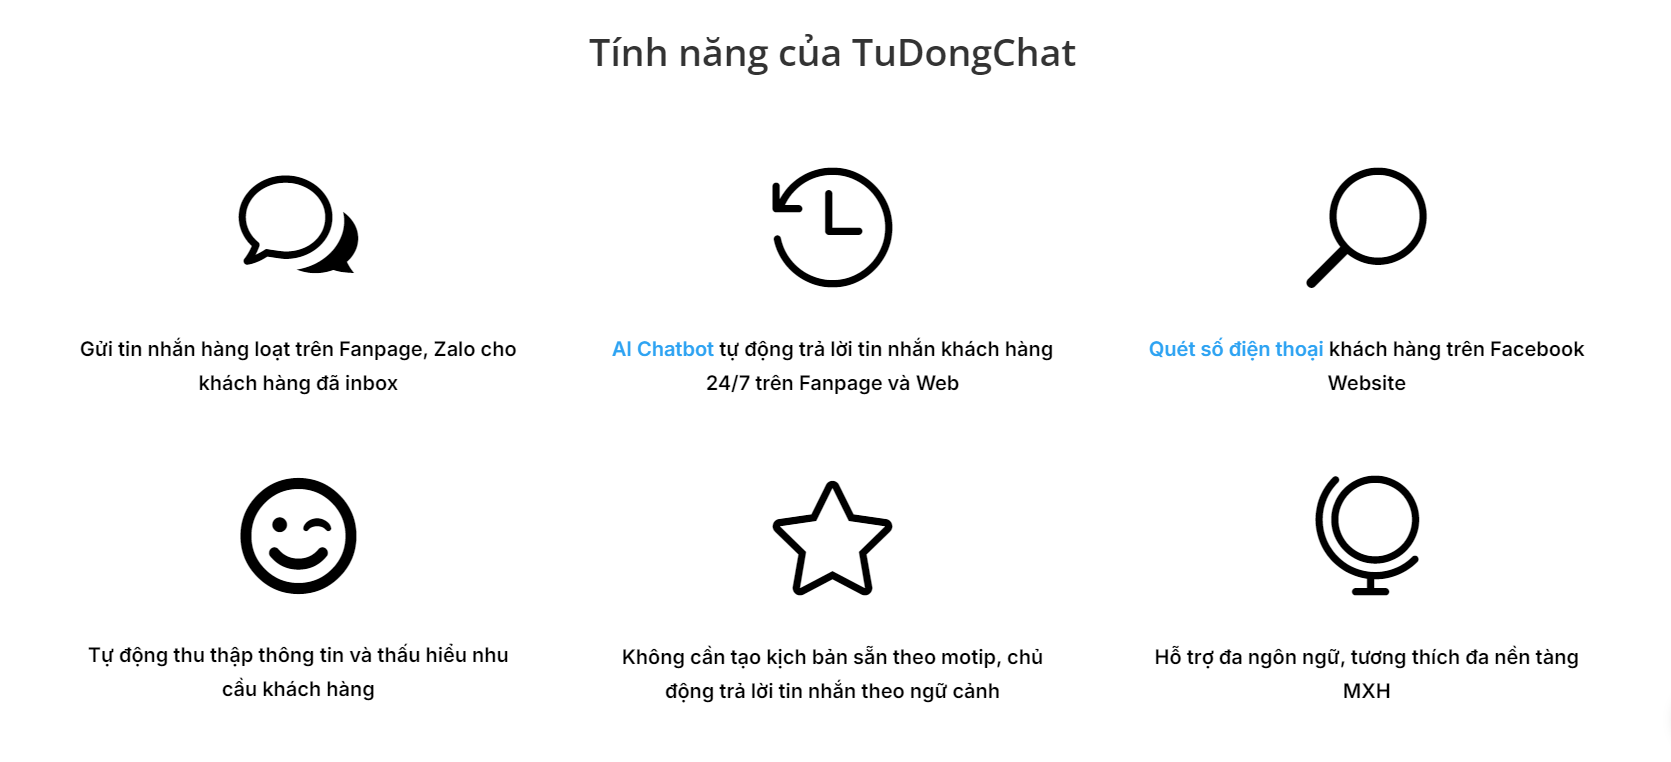
\includegraphics[width=1\linewidth]{Images/tinhnangtudongchat.png}
    \vspace{0.5cm}
    \caption{Các tính năng cơ bản của TuDongChat}
    \label{fig:enter-label}
\end{figure}
\subsubsection{Phân tích SWOT}
\begin{table}[H]
\centering
\begin{tabular}{|p{7cm}|p{7cm}|}
\hline
\begin{center}
    Strengths
\end{center}
  &  \begin{center}
      Weaknesses
  \end{center} \\
\hline
\begin{itemize}
    \item Hỗ trợ tạo chatbot tự động cho doanh nghiệp mà không yêu cầu kỹ năng lập trình.
\item Tính năng tích hợp đa kênh từ Facebook Messenger, Zalo đến website.
\item Giao diện quản lý đơn giản và tập trung vào tự động hóa các tác vụ liên quan đến chăm sóc khách hàng.

\end{itemize} &  
\begin{itemize}
    \item Tính năng chưa đa dạng bằng các nền tảng lớn khác, hạn chế trong việc tùy chỉnh các kịch bản phức tạp.
\item Thiếu các công cụ phân tích sâu sắc để theo dõi hành vi khách hàng và hiệu quả chatbot.
\end{itemize}\\
\hline
\begin{center}
    Opportunities
\end{center} & \begin{center}
    Threats
\end{center}\\
\hline
\begin{itemize}
    \item Tăng trưởng của thị trường chatbot tại Việt Nam, đặc biệt trong các ngành bán lẻ và dịch vụ.
\item Cơ hội phát triển và mở rộng thêm tính năng tự động hóa nâng cao và tích hợp với nhiều nền tảng khác.
\end{itemize} &  
\begin{itemize}
    \item Sự xuất hiện của các đối thủ cạnh tranh lớn trong nước và quốc tế với nhiều tính năng hơn.
\item Công nghệ phát triển nhanh chóng đòi hỏi liên tục đổi mới để theo kịp xu hướng.
\end{itemize}\\
\hline
\end{tabular}
\caption{Bảng phân tích SWOT cho hệ thống TuDongChat}
\end{table}
\newpage
\section{Phân tích hệ thống}
\subsection{Stakeholders}
\subsubsection{Đội phát triển phần mềm}

Nhóm phát triển phần mềm chịu trách nhiệm xây dựng, thử nghiệm và triển khai sản phẩm theo các yêu cầu được cung cấp.

\begin{itemize}
    \item \textbf{Nhu cầu:}
    \begin{itemize}
        \item Nhóm cần có phạm vi dự án và các yêu cầu được xác định rõ ràng để đảm bảo lập kế hoạch hiệu quả và đồng nhất với các mục tiêu được đặt ra.
        \item Nhóm cần được tạo điều kiện tiếp cận các công cụ và công nghệ cần thiết để thực hiện nhiệm vụ của mình một cách hiệu quả và sáng tạo.
    \end{itemize}
    \item \textbf{Ảnh hưởng:} Nhóm phát triển có ảnh hưởng lớn do nhóm tham gia trực tiếp vào quá trình thực hiện dự án. Công việc của nhóm tác động trực tiếp đến chất lượng và chức năng của sản phẩm cuối cùng, khiến cho sự đóng góp và sự hài lòng của nhóm phát triển quan trọng đối với sự thành công của dự án.
\end{itemize}

\subsubsection{Các doanh nghiệp khách hàng}

Đây là những doanh nghiệp sử dụng hệ thống để tạo và triển khai chatbot AI trên trang web của họ.

\begin{itemize}
    \item \textbf{Nhu cầu:}
    \begin{itemize}
        \item Khách hàng cần một giao diện trực quan và tích hợp liền mạch để tăng hiệu quả và giảm thiểu thời gian triển khai.
        \item Chatbot cần có khả năng tùy chỉnh giao diện để phù hợp với nhận diện thương hiệu của khách hàng.
        \item Chức năng của chatbot cần đáng tin cậy và hiệu suất cao để duy trì sự hài lòng của người dùng.
        \item Hệ thống cần đảm bảo bảo vệ dữ liệu và tuân thủ các quy định liên quan.
        \item Cần có kênh hỗ trợ nhanh chóng và tài liệu hướng dẫn chi tiết giúp khách hàng sử dụng nền tảng một cách hiệu quả.
        \item Giá cả rõ ràng và hợp lý giúp khách hàng quản lý ngân sách hợp lý.
    \end{itemize}
    \item \textbf{Ảnh hưởng:} Các công ty khách hàng có ảnh hưởng lớn vì các yêu cầu của họ định hình mạnh mẽ các tính năng và chức năng của sản phẩm. Phản hồi và nhu cầu của họ định hình nên hướng phát triển của hệ thống.
\end{itemize}

\subsubsection{Người dùng cuối (Khách hàng của các doanh nghiệp khách hàng)}

Đây là những cá nhân tương tác với chatbot trên trang web của khách hàng nhằm tìm kiếm thông tin hoặc có nhu cầu hỗ trợ.

\begin{itemize}
    \item \textbf{Nhu cầu:}
    \begin{itemize}
        \item Chatbot cần có khả năng phản hồi nhanh chóng và chính xác cho các truy vấn.
        \item Tương tác với chatbot được cá nhân hóa, cải thiện mức độ tương tác và trải nghiệm của người dùng.
        \item Hệ thống cần đảm bảo quyền riêng tư và bảo mật dữ liệu của người dùng.
        \item Có khả năng chuyển đối tượng giao tiếp AI qua con người để đảm bảo hỗ trợ toàn diện.
    \end{itemize}
    \item \textbf{Ảnh hưởng:} Người dùng cuối có ảnh hưởng trực tiếp thấp nhưng tác động gián tiếp đến dự án thông qua hành vi sử dụng và phản hồi của họ, thông tin này cũng sẽ định hình cho các cải tiến của hệ thống.
\end{itemize}

\subsubsection{Nhóm hỗ trợ khách hàng tại doanh nghiệp khách hàng}

Các nhóm này xử lý các yêu cầu phức tạp của khách hàng và quản lý các tương tác được chuyển tiếp từ chatbot.

\begin{itemize}
    \item \textbf{Nhu cầu:}
    \begin{itemize}
        \item Hệ thống có khả năng chuyển đổi liền mạch giữa chatbot và các tác nhân con người để duy trì chất lượng dịch vụ.
        \item Cho phép truy cập vào lịch sử hội thoại và phân tích, từ đó hiểu các vấn đề của khách hàng và cải thiện dịch vụ.
        \item Cần có công cụ giám sát hiệu suất chatbot để đảm bảo chatbot hoạt động tối ưu.
        \item Cần có hình thức đào tạo phù hợp đảm bảo rằng nhóm hỗ trợ có thể tận dụng tối đa khả năng của hệ thống.
    \end{itemize}
    \item \textbf{Ảnh hưởng:} Các nhóm hỗ trợ khách hàng có ảnh hưởng trung bình vì phản hồi và kinh nghiệm của họ ảnh hưởng đến khả năng sử dụng và hiệu quả của hệ thống.
\end{itemize}

\subsubsection{Quản trị viên hệ thống (nội bộ và phía khách hàng)}

Quản trị viên hệ thống chịu trách nhiệm quản lý cấu hình, bảo trì và bảo mật hệ thống.

\begin{itemize}
    \item \textbf{Nhu cầu:}
    \begin{itemize}
        \item Quyền kiểm soát quản trị và bảng thông tin toàn diện, đầy đủ là cần thiết để quản lý hệ thống hiệu quả.
        \item Hệ thống có tính ổn định và thời gian hoạt động cao là rất quan trọng.
        \item Hệ thống phải có khả năng mở rộng và hoạt động tối ưu khi mức sử dụng tăng lên.
        \item Việc tuân thủ các chính sách bảo mật và công nghệ thông tin là cần thiết để bảo vệ dữ liệu nhạy cảm và duy trì tính toàn vẹn của hệ thống.
    \end{itemize}
    \item \textbf{Ảnh hưởng:} Quản trị viên hệ thống có ảnh hưởng cao do vai trò quan trọng của họ trong việc triển khai kỹ thuật và đảm bảo tuân thủ các tiêu chuẩn bảo mật.
\end{itemize}

\subsubsection{Nhóm đào tạo và hỗ trợ}

Các nhóm này chịu trách nhiệm cung cấp dịch vụ hướng dẫn, đào tạo và hỗ trợ liên tục cho các công ty khách hàng.

\begin{itemize}
    \item \textbf{Nhu cầu:}
    \begin{itemize}
        \item Phát triển tài liệu hướng dẫn toàn diện, chi tiết giúp khách hàng hiểu và sử dụng nền tảng hiệu quả.
        \item Giải quyết hiệu quả các vấn đề và thắc mắc: Hỗ trợ nhanh chóng và hiệu quả là điều cần thiết để duy trì lòng tin của khách hàng.
        \item Thu thập phản hồi để cải tiến liên tục: Thu thập phản hồi giúp tinh chỉnh các quy trình đào tạo và hỗ trợ.
    \end{itemize}
    \item \textbf{Ảnh hưởng:} Các nhóm đào tạo và hỗ trợ có ảnh hưởng từ thấp đến trung bình, chủ yếu thông qua tác động của họ đến tỷ lệ áp dụng và sự hài lòng của khách hàng thông qua hiệu quả đào tạo.
\end{itemize}


\subsection{Yêu cầu chức năng}

\subsubsection{Quản lý tài khoản công ty}

\paragraph{Đăng ký và xác thực}
\begin{itemize}
    \item Hệ thống sẽ cung cấp quy trình đăng ký tài khoản mới an toàn cho các công ty.
    \item Hệ thống sẽ yêu cầu xác minh địa chỉ email trong quá trình đăng ký.
    \item Hệ thống sẽ hỗ trợ chức năng đăng nhập an toàn bằng tên người dùng/email và mật khẩu.
\end{itemize}

\paragraph{Quản lý hồ sơ}
\begin{itemize}
    \item Hệ thống sẽ cho phép quản trị viên công ty quản lý thông tin chi tiết về hồ sơ công ty (tên, logo, thông tin liên hệ…).
    \item Hệ thống sẽ cho phép quản trị viên công ty quản lý vai trò và quyền của người dùng trong tài khoản công ty của họ.
    \item Hệ thống sẽ cho phép công ty cập nhật hồ sơ cá nhân và cài đặt tài khoản của họ.
    \item Hệ thống sẽ cho phép người dùng đặt lại mật khẩu an toàn.
\end{itemize}

\subsubsection{Tạo và tùy chỉnh chatbot}

\paragraph{Cung cấp và quản lý tri thức}
\begin{itemize}
    \item Hệ thống sẽ cho phép các công ty tải dữ liệu của riêng họ lên, ví dụ như tài liệu, các câu hỏi thường gặp (FAQs) hay thông tin sản phẩm.
    \item Hệ thống sẽ hỗ trợ nhiều định dạng tệp để tải dữ liệu lên, chẳng hạn như PDF, DOCX, TXT và CSV.
    \item Hệ thống sẽ xử lý dữ liệu đã tải lên để tạo cơ sở tri thức cho chatbot.
    \item Hệ thống sẽ cho phép các công ty thêm, chỉnh sửa hoặc xóa các tri thức thông qua giao diện.
    \item Hệ thống sẽ cho phép phân loại và gắn thẻ nội dung cơ sở tri thức để truy vấn hiệu quả.
\end{itemize}

\paragraph{Tùy chỉnh giao diện và hành vi chatbot}
\begin{itemize}
    \item Hệ thống sẽ cho phép các công ty điều chỉnh giọng điệu và tính cách của chatbot (ví dụ: trang trọng, giản dị, thân thiện).
    \item Hệ thống sẽ cho phép tùy chỉnh lời chào và phản hồi mặc định của chatbot.
    \item Hệ thống sẽ cung cấp các tùy chọn để tùy chỉnh giao diện của chatbot, bao gồm màu sắc, logo, hình đại diện để phù hợp với thương hiệu của công ty.
    \item Hệ thống sẽ cung cấp chức năng xem trước để xem các thay đổi trước khi triển khai.
\end{itemize}

\subsubsection{Đào tạo AI và xử lý ngôn ngữ tự nhiên}

\paragraph{Đào tạo tự động}
\begin{itemize}
    \item Hệ thống sẽ tự động đào tạo mô hình AI bằng cách sử dụng dữ liệu công ty đã tải lên.
    \item Hệ thống sẽ thông báo tiến độ trong quá trình đào tạo.
\end{itemize}

\paragraph{Xử lý ngôn ngữ tự nhiên}
\begin{itemize}
    \item Hệ thống sẽ hỗ trợ tiếng Việt cho cả đầu vào và phản hồi.
    \item Mô hình AI sẽ sử dụng hiểu ngôn ngữ tự nhiên (Natural-language understanding) để nhận dạng chính xác ý định người dùng.
    \item Hệ thống sẽ cho phép các công ty xác định các ý định cụ thể có liên quan đến doanh nghiệp của họ.
\end{itemize}

\subsubsection{Tích hợp với trang web doanh nghiệp}

\paragraph{Tích hợp mã nhúng}
\begin{itemize}
    \item Hệ thống sẽ tạo mã nhúng JavaScript mà các công ty có thể chèn vào trang web của họ để triển khai chatbot.
    \item Hệ thống sẽ cung cấp hướng dẫn từng bước để tích hợp chatbot với các nền tảng và trình xây dựng trang web phổ biến như WordPress, Wix, Shopify.
    \item Mã nhúng sẽ được tối ưu hóa để tác động tối thiểu đến hiệu suất của trang web.
\end{itemize}

\paragraph{Khả năng tương thích của nền tảng}
\begin{itemize}
    \item Giao diện chatbot phải tương thích với tất cả các trình duyệt web hiện đại (Chrome, Firefox, Safari, Edge).
    \item Chatbot phải phản hồi và hoạt động chính xác trên nhiều thiết bị khác nhau, bao gồm máy tính để bàn, máy tính bảng và điện thoại di động.
\end{itemize}

\subsubsection{Bảng điều khiển quản lý Chatbot}

\paragraph{Giám sát thời gian thực}
\begin{itemize}
    \item Hệ thống sẽ cung cấp bảng điều khiển để các công ty xem dữ liệu theo thời gian thực về việc sử dụng chatbot, bao gồm số lượng người dùng đang hoạt động và các cuộc trò chuyện đang diễn ra.
    \item Hệ thống sẽ hiển thị các chỉ số hiệu suất chính (KPI) như thời gian phản hồi và mức độ tương tác của người dùng.
\end{itemize}

\paragraph{Phân tích và báo cáo}
\begin{itemize}
    \item Hệ thống sẽ tạo báo cáo phân tích chi tiết về các tương tác của chatbot, bao gồm tổng số cuộc trò chuyện, tỷ lệ giữ chân người dùng và các truy vấn phổ biến.
    \item Hệ thống sẽ cho phép các công ty xuất báo cáo ở nhiều định dạng khác nhau (ví dụ: PDF, Excel).
    \item Hệ thống sẽ cung cấp các công cụ trực quan hóa (biểu đồ, đồ thị) giúp trực quan hóa dữ liệu.
\end{itemize}

\paragraph{Nhật ký hội thoại}
\begin{itemize}
    \item Hệ thống sẽ lưu trữ lịch sử cuộc trò chuyện một cách an toàn.
    \item Hệ thống sẽ cho phép người dùng được ủy quyền tìm kiếm và lọc nhật ký hội thoại dựa trên phạm vi ngày, từ khóa hoặc chủ đề.
    \item Hệ thống phải tuân thủ các quy định về quyền riêng tư liên quan đến việc lưu trữ và truy xuất các cuộc trò chuyện của người dùng.
\end{itemize}

\subsubsection{Tương tác với người dùng}

\paragraph{Hỗ trợ đa phương tiện}
\begin{itemize}
    \item Chatbot phải có khả năng gửi và nhận nội dung đa phương tiện, bao gồm hình ảnh, video và đường dẫn (hyperlinks).
\end{itemize}

\paragraph{Đối thoại theo ngữ cảnh}
\begin{itemize}
    \item Chatbot phải duy trì ngữ cảnh trong suốt phiên của người dùng để cho phép các cuộc trò chuyện diễn ra mạch lạc.
    \item Chatbot phải có khả năng xử lý các câu hỏi tiếp theo và tham chiếu đến các tương tác trước đó.
\end{itemize}

\paragraph{Khôi phục và dự phòng}
\begin{itemize}
    \item Chatbot phải cung cấp các phản hồi mặc định phù hợp khi không hiểu nội dung đầu vào của người dùng.
    \item Chatbot phải cung cấp các tùy chọn để người dùng diễn đạt lại truy vấn của họ hoặc cung cấp thêm thông tin.
\end{itemize}

\subsubsection{Phối hợp với con người}

\paragraph{Tích hợp với nhân viên hỗ trợ trực tiếp}
\begin{itemize}
    \item Hệ thống sẽ cho phép chuyển giao liền mạch các cuộc trò chuyện từ chatbot sang nhân viên hỗ trợ con người khi cần thiết.
    \item Hệ thống sẽ thông báo cho nhân viên hỗ trợ theo thời gian thực khi cần chuyển giao.
    \item Hệ thống sẽ cung cấp cho nhân viên lịch sử cuộc trò chuyện trước khi chuyển giao để đảm bảo duy trì ngữ cảnh.
\end{itemize}

\paragraph{Đặt lịch hẹn}
\begin{itemize}
    \item Hệ thống sẽ cho phép các công ty cài đặt lịch làm việc của nhân viên để hỗ trợ con người.
    \item Chatbot sẽ thông báo cho người dùng về lịch làm việc của nhân viên và thời gian phản hồi ước tính.
    \item Ngoài giờ làm việc, chatbot sẽ đề nghị hẹn lịch hoặc cung cấp các thông tin liên hệ.
\end{itemize}

\subsubsection{Thông báo và cảnh báo}

\begin{itemize}
    \item Hệ thống sẽ gửi email hoặc thông báo đến doanh nghiệp khi cần thiết (hoàn thành đào tạo AI, nhắc gia hạn đăng ký).
    \item Hệ thống sẽ cho phép các công ty tùy chỉnh phương thức thông báo.
    \item Hệ thống sẽ cho phép các công ty thiết lập cảnh báo dựa trên số liệu hiệu suất (ví dụ: lưu lượng truy cập cao, tỷ lệ lỗi).
    \item Hệ thống sẽ lập tức cảnh báo trong trường hợp hệ thống ngừng hoạt động hoặc các sự cố nghiêm trọng.
\end{itemize}

\subsubsection{Hỗ trợ doanh nghiệp}
\begin{itemize}
    \item Hệ thống sẽ cung cấp một trung tâm trợ giúp toàn diện với các tài liệu, câu hỏi thường gặp và hướng dẫn sử dụng nền tảng.
    \item Hệ thống sẽ bao gồm chức năng tìm kiếm để giúp người dùng tìm thông tin hỗ trợ có liên quan một cách nhanh chóng.
    \item Hệ thống sẽ cung cấp nhiều kênh hỗ trợ khách hàng, bao gồm trò chuyện trực tiếp, email và hỗ trợ qua điện thoại.
\end{itemize}

\subsubsection{Quản lý thanh toán}

\paragraph{Gói giá linh hoạt}
\begin{itemize}
    \item Hệ thống sẽ cung cấp nhiều cấp đăng ký với các tính năng và giới hạn sử dụng khác nhau.
    \item Hệ thống sẽ cho phép các công ty nâng cấp hoặc hạ cấp các gói đăng ký của họ khi cần.
\end{itemize}

\paragraph{Xử lý thanh toán}
\begin{itemize}
    \item Hệ thống sẽ tích hợp với các cổng thanh toán an toàn để xử lý các giao dịch bằng nhiều phương thức thanh toán khác nhau.
    \item Hệ thống sẽ hỗ trợ thanh toán định kỳ tự động cho các lần gia hạn đăng ký.
\end{itemize}

\paragraph{Theo dõi việc sử dụng và lập hóa đơn}
\begin{itemize}
    \item Hệ thống sẽ tạo hóa đơn và cung cấp hồ sơ giao dịch mà các công ty có thể truy cập.
    \item Hệ thống sẽ theo dõi các số liệu sử dụng ảnh hưởng đến việc thanh toán, chẳng hạn như số lần tương tác hoặc dung lượng lưu trữ dữ liệu đã sử dụng.
\end{itemize}

\subsection{Yêu cầu phi chức năng}

\subsubsection{Hiệu suất}

\paragraph{Thời gian phản hồi}
\begin{itemize}
    \item Hệ thống phải đảm bảo rằng chatbot phản hồi người dùng trong vòng trung bình 3 giây trong điều kiện tải bình thường.
    \item Hệ thống phải duy trì thời gian phản hồi tối đa là 5 giây trong thời gian tải cao điểm.
\end{itemize}

\paragraph{Thông lượng}
\begin{itemize}
    \item Hệ thống phải hỗ trợ ít nhất 500 người dùng đồng thời mà không làm giảm hiệu suất.
    \item Hệ thống phải xử lý 100 giao dịch mỗi giây (TPS) trong thời gian sử dụng cao điểm.
\end{itemize}

\paragraph{Khả năng mở rộng}
\begin{itemize}
    \item Hệ thống phải có khả năng mở rộng để đáp ứng mức tăng 25\% về số lượng công ty khách hàng hàng năm mà không cần thiết kế lại đáng kể.
    \item Hệ thống phải tự động mở rộng tài nguyên (tính toán, lưu trữ) dựa trên nhu cầu thời gian thực.
\end{itemize}

\paragraph{Tính khả dụng}
\begin{itemize}
    \item Hệ thống phải có thời gian hoạt động ít nhất là 99\%, không bao gồm bảo trì theo lịch trình.
    \item Thời gian bảo trì theo lịch trình không được vượt quá 6 giờ mỗi tháng và phải được thông báo cho khách hàng trước ít nhất 24 giờ.
\end{itemize}

\subsubsection{Bảo mật}

\paragraph{Xác thực và ủy quyền}
\begin{itemize}
    \item Hệ thống phải thực thi các chính sách mật khẩu mạnh (yêu cầu về độ dài tối thiểu, độ phức tạp).
    \item Hệ thống phải hỗ trợ xác thực đa yếu tố (MFA) cho tất cả tài khoản người dùng.
    \item Kiểm soát truy cập dựa trên vai trò (RBAC) phải được triển khai để hạn chế quyền truy cập dựa trên vai trò của người dùng.
\end{itemize}

\paragraph{Bảo mật dữ liệu}
\begin{itemize}
    \item Tất cả dữ liệu đang truyền đi phải được mã hóa bằng các giao thức tiêu chuẩn của ngành từ TLS 1.2 trở lên.
    \item Dữ liệu nhạy cảm khi lưu trữ phải được mã hóa nếu có thể hoặc được lưu trữ an toàn bằng biện pháp kiểm soát truy cập.
    \item Hệ thống phải triển khai các đánh giá bảo mật và quét lỗ hổng thường xuyên.
    \item Hệ thống phải tuân thủ các quy định bảo vệ dữ liệu cơ bản áp dụng cho khu vực mà hệ thống hoạt động.
    \item Hệ thống phải cung cấp chính sách bảo mật nêu rõ các hoạt động xử lý dữ liệu.
\end{itemize}

\paragraph{Phản hồi sự cố}
\begin{itemize}
    \item Hệ thống sẽ có kế hoạch phản hồi sự cố để giải quyết các vi phạm bảo mật hoặc rò rỉ dữ liệu.
    \item Các sự cố bảo mật sẽ được báo cáo cho các khách hàng bị ảnh hưởng trong vòng 72 giờ kể từ khi phát hiện.
\end{itemize}

\subsubsection{Khả năng sử dụng}

\paragraph{Giao diện người dùng}
\begin{itemize}
    \item Hệ thống phải có giao diện thân thiện với người dùng, tập trung vào tính dễ sử dụng cho người dùng không chuyên.
    \item Giao diện phải nhất quán và trực quan, tuân theo các nguyên tắc cơ bản.
\end{itemize}

\paragraph{Khả năng truy cập}
\begin{itemize}
    \item Hệ thống phải tuân thủ các tiêu chuẩn về khả năng truy cập WCAG 2.0 A để hỗ trợ người dùng khuyết tật.
    \item Các yếu tố tương tác chính có thể được thực hiện thông qua bàn phím.
\end{itemize}

\paragraph{Trợ giúp và tài liệu hướng dẫn}
\begin{itemize}
    \item Hệ thống sẽ cung cấp tài liệu hướng dẫn và các câu hỏi thường gặp có thể truy cập từ bên trong nền tảng.
    \item Tài liệu phải rõ ràng và được cập nhật để phản ánh hệ thống hiện tại.
\end{itemize}

\subsubsection{Độ tin cậy}

\paragraph{Khả năng chịu lỗi}
\begin{itemize}
    \item Hệ thống sẽ tiếp tục hoạt động bình thường trong trường hợp các thành phần không quan trọng bị lỗi.
    \item Hệ thống sẽ ghi lại lỗi và thông báo cho người quản trị trong trường hợp lỗi nghiêm trọng.
\end{itemize}

\paragraph{Sao lưu và phục hồi}
\begin{itemize}
    \item Hệ thống sẽ thực hiện sao lưu tự động hàng tuần tất cả dữ liệu quan trọng.
    \item Trong trường hợp xảy ra lỗi, hệ thống sẽ có thể khôi phục dữ liệu về điểm sao lưu cuối cùng trong vòng 8 giờ.
    \item Các bản sao lưu sẽ được lưu trữ an toàn và được bảo vệ khỏi truy cập trái phép.
\end{itemize}

\paragraph{Xử lý lỗi}
\begin{itemize}
    \item Hệ thống sẽ xử lý lỗi một cách nhẹ nhàng, cung cấp thông báo thân thiện với người dùng mà không tiết lộ chi tiết kỹ thuật.
    \item Tất cả các lỗi quan trọng sẽ được ghi lại để phục vụ mục đích khắc phục sự cố.
\end{itemize}

\subsubsection{Khả năng bảo trì}

\paragraph{Tính mô-đun}
\begin{itemize}
    \item Hệ thống sẽ được thiết kế mô-đun hóa khi có thể, để tạo điều kiện thuận lợi cho việc mở rộng và bảo trì.
    \item Mã nguồn được sắp xếp hợp lý và ghi chú đầy đủ để thuận tiện bảo trì.
\end{itemize}

\paragraph{Kiểm thử}
\begin{itemize}
    \item Hệ thống sẽ có các bài kiểm thử tự động cho các chức năng chính.
    \item Kiểm thử tích hợp sẽ được thực hiện trước khi triển khai.
\end{itemize}

\subsubsection{Tính di động}

\paragraph{Độc lập với nền tảng}
\begin{itemize}
    \item Hệ thống sẽ sử dụng các công nghệ được hỗ trợ rộng rãi để đảm bảo khả năng tương thích trên các nền tảng phổ biến.
    \item Mã nhúng chatbot sẽ hoạt động chính xác trên các môi trường web.
\end{itemize}

\paragraph{Khả năng tương thích với trình duyệt}
\begin{itemize}
    \item Giao diện chatbot sẽ tương thích với các phiên bản mới nhất của các trình duyệt web chính.
    \item Hệ thống sẽ được thử nghiệm trên Chrome, Edge và Firefox.
\end{itemize}

\subsubsection{Yêu cầu về mặt pháp lý}

\paragraph{Quyền riêng tư dữ liệu}
\begin{itemize}
    \item Hệ thống chỉ thu thập dữ liệu cá nhân cần thiết và thông báo cho người dùng về các hoạt động thu thập dữ liệu.
    \item Người dùng phải đồng ý thu thập dữ liệu khi cần thiết.
\end{itemize}

\paragraph{Kiểm toán và báo cáo}
\begin{itemize}
    \item Hệ thống phải lưu giữ nhật ký cơ bản về các hành động của quản trị viên.
    \item Nhật ký phải được lưu giữ trong ít nhất 6 tháng.
\end{itemize}

\paragraph{Sở hữu trí tuệ}
\begin{itemize}
    \item Hệ thống phải đảm bảo tất cả phần mềm và nội dung của bên thứ ba đều có giấy phép phù hợp.
\end{itemize}

\subsubsection{Đạo đức}

\paragraph{Minh bạch AI}
\begin{itemize}
    \item Chatbot sẽ thông báo cho người dùng rằng họ đangtương tác với trợ lý AI.
    \item Chatbot không được đánh lừa người dùng nghĩ rằng đó là con người.
\end{itemize}

\paragraph{Bảo vệ người dùng}
\begin{itemize}
    \item Chatbot phải tránh tạo ra các nội dung nhạy cảm, gây khó chịu.
    \item Chatbot phải khuyên người dùng không chia sẻ thông tin cá nhân nhạy cảm.
    \item Hệ thống sẽ cung cấp phương pháp để người dùng báo cáo các phản hồi không phù hợp.
\end{itemize}
\subsection{Biểu đồ Use case}
Vẽ biểu đồ use case và use case scenario
\subsection{Biểu đồ Activity}
\subsection{Biểu đồ Sequence}
\subsection{Biểu đồ Class}

\newpage
\section{Thiết kế hệ thống}
\subsection{Kiến trúc hệ thống}
Mô tả kiến trúc chi tiết từng thành phần, biện luận vì sao dùng cho hệ thống ta
\subsection{Cơ sở dữ liệu}
Vẽ lược đồ ERD, phân tích các entity và relation có thể có trong hệ thống
\subsection{Giao diện}
Bản đồ các giao diện của phần mềm
Chi tiết từng giao diện 
\newpage
\section{Hiện thực}
\subsection{Công nghệ}
Kỹ thuật, công nghệ, tóm tắt mô tả

Vẽ, Mô tả kiến trúc khi hiện thực, thành phần chức năng gì khi tương tác vs nhau
\subsection{Các tính năng chính}
Hiện thực một vài tính năng của hệ thống


\newpage
% Đồ án tốt nghiệp
% \section{Kiểm thử hệ thống}
Đưa ra các testcase để kiểm thử hệ thống, và kết quả test
% \newpage
% \section{Triển khai}
Deployment
% \newpage
\section{Tổng kết}
\subsection{Nhận xét}
\subsection{Hướng phát triển}
%%%%%%%%%%%%%%%%%OUTRO%%%%%%%%%%%%%%%%%%%
\section{Tài liệu tham khảo}
\newpage
\section{Phụ lục}
\end{document}


